


\documentclass[12pt,a4paper,oneside]{book}





\usepackage[utf8]{inputenc}
\usepackage[T1]{fontenc}
\usepackage[italian]{babel}

\usepackage[a4paper,inner=3.5cm,outer=2.5cm,top=3cm,bottom=3cm]{geometry}
\usepackage{fancyhdr}
\usepackage{indentfirst}
\usepackage{parskip}
\usepackage{emptypage}

\usepackage{microtype}
\usepackage{hyphenat}
\hyphenation{mate-mati-ca recu-perare}

\usepackage[titletoc,title,toc,page]{appendix}
\usepackage{chngcntr}
\counterwithin{table}{chapter}
\counterwithin{figure}{chapter}

\usepackage{amsmath}
\usepackage{amssymb}

\usepackage{graphicx}
\usepackage{float}
\usepackage{placeins}
\usepackage{lscape}
\usepackage{tikz}
\usepackage{pgfplots}
\pgfplotsset{compat=1.18}
\usetikzlibrary{shapes.geometric, arrows.meta, positioning}

\usepackage{pdfpages}

\usepackage{multirow}
\usepackage{booktabs}
\usepackage[font=footnotesize,labelfont=bf]{caption}

\usepackage{listings}
\usepackage{verbatim}

\lstset{
    basicstyle=\ttfamily\small,
    breaklines=true,
    frame=single,
    numbers=left,
    numberstyle=\tiny,
    keywordstyle=\bfseries,
    commentstyle=\itshape,
    stringstyle=\ttfamily,
    captionpos=b,
    showstringspaces=false,
    inputencoding=utf8,
    extendedchars=true,
    literate={à}{{\`a}}1 {è}{{\`e}}1 {ì}{{\`\i}}1 {ò}{{\`o}}1 {ù}{{\`u}}1
        {À}{{\`A}}1 {È}{{\`E}}1 {Ì}{{\`I}}1 {Ò}{{\`O}}1 {Ù}{{\`U}}1,
}

\usepackage{xcolor}
\usepackage{listings}

\definecolor{codegreen}{rgb}{0.13,0.55,0.13}
\definecolor{codegray}{rgb}{0.5,0.5,0.5}
\definecolor{codepurple}{rgb}{0.58,0,0.82}
\definecolor{backcolour}{rgb}{0.96,0.96,0.96}
\definecolor{codeblue}{rgb}{0.0,0.0,0.8}
\definecolor{codeorange}{rgb}{0.9,0.4,0.0}

\lstset{
    backgroundcolor=\color{backcolour},   
    commentstyle=\color{codegreen},
    keywordstyle=\color{codeblue}\bfseries,
    numberstyle=\tiny\color{codegray},
    stringstyle=\color{codepurple},
    basicstyle=\ttfamily\small,
    breakatwhitespace=false,         
    breaklines=true,                 
    captionpos=b,                    
    keepspaces=true,                 
    numbers=left,                    
    numbersep=5pt,                  
    showspaces=false,                
    showstringspaces=false,
    showtabs=false,                  
    tabsize=4
}

\addto\captionsitalian{\renewcommand{\lstlistingname}{Code}\renewcommand{\lstlistlistingname}{Elenco dei codici}}

\lstdefinelanguage{TypeScript}{
    keywords={abstract, any, as, asconst, boolean, break, case, catch, class, console, const, continue, debugger, declare, default, delete, do, else, enum, export, extends, false, finally, for, from, function, get, if, implements, import, in, instanceof, interface, is, keyof, let, module, namespace, never, new, null, number, object, package, private, protected, public, readonly, require, return, set, static, string, super, switch, this, throw, true, try, type, typeof, unknown, var, void, while, with, yield},
    morecomment=[l]{//},
    morecomment=[s]{/*}{*/},
    morestring=[b]',
    morestring=[b]", morestring=[b]`
}
\lstdefinelanguage{Sparql}{
    keywords={SELECT, WHERE, FILTER, OPTIONAL, UNION, PREFIX, BASE},
    morecomment=[l]{\#},
    morestring=[b]',
    morestring=[b]", morestring=[b]`
}
\lstdefinelanguage{Python}{
    keywords={import, as, def, class, return, if, else, for, in, while, try, except, finally, with, from, yield, pass, break, continue, global, nonlocal},
    morecomment=[l]{\#},
    morestring=[b]',
    morestring=[b]", }
\lstdefinelanguage{txt}{
    keywords={},
}



\usepackage{etoolbox}
\usepackage[most]{tcolorbox} 
\usepackage{xcolor}
\definecolor{mygray}{RGB}{200,200,200}
\usepackage{newlfont}
\usepackage{soul}
\usepackage{enumitem}
\usepackage{tabularx}
\usepackage{xltabular}
\usepackage{multicol}

\definecolor{light-gray}{gray}{0.95}


\newtcolorbox{mybox}[1][]{blanker, 
    left skip=1.3em,
    left=-1.3em,
    borderline west={1.5pt}{0pt}{gray},
    breakable,
    #1}

\AtBeginEnvironment{quotation}{\begin{mybox}}
\AtEndEnvironment{quotation}{\end{mybox}}
\AtBeginEnvironment{quote}{\begin{mybox}}
\AtEndEnvironment{quote}{\end{mybox}}

\usepackage[hidelinks,
            pdftitle={Titolo della Tesi},
            pdfauthor={Alberto Zuccari},
            pdfsubject={Tesi di Laurea},
            pdfkeywords={parola1, parola2, parola3}]{hyperref}
\usepackage{cleveref}

\crefname{section}{paragrafo}{paragrafi}
\crefname{chapter}{capitolo}{capitoli}
\crefname{subsection}{paragrafo}{paragrafi}
\crefname{subsubsection}{paragrafo}{paragrafi}
\crefname{figure}{figura}{figure}
\crefname{table}{tabella}{tabella}
\crefname{equation}{equazione}{equazioni}
\crefname{listing}{listing}{listing}
\crefname{theorem}{teorema}{teoremi}
\crefname{lemma}{lemma}{lemma}
\crefname{proof}{prova}{prove}
\crefname{corollary}{corollario}{corollari}
\crefname{remark}{nota}{note}
\crefname{example}{esempio}{esempi}





\newcommand{\rom}[1]{\MakeUppercase{\romannumeral#1\relax}}
\newcommand{\code}[1]{\colorbox{light-gray}{\texttt{#1}}}

\newcommand{\var}{\texttt}

\newcommand{\myfootnotemark}{\stepcounter{footnote}\footnotemark[\thefootnote]\setcounter{mycount}{\value{footnote}}}
\newcommand{\firstfootnotetext}[1]{\footnotetext[\themycount]{#1}}
\newcommand{\otherfootnotetext}[1]{\stepcounter{mycount}\footnotetext[\themycount]{#1}}




\usepackage[numbers]{natbib}
\bibliographystyle{alpha}





\begin{document}




\pagenumbering{roman}
\pagestyle{empty}
\newgeometry{left=20mm, right=20mm, top=20mm, bottom=20mm}

\begin{titlepage}
\begin{center}


\includegraphics[width=6.5cm,height=4.7cm]{../img/marchio-di-ateneo.png}

\vspace{10mm}

{\large{\bf{Dipartimento di Informatica Scienza e Ingegneria}}}

\vspace{5mm}

{\Large{\bf{Corso di Laurea in Informatica}}}

\vspace{15mm}

{\Huge{\bf Traduzione da linguaggio naturale}}\\
\vspace{3mm}
{\Huge{\bf a query per Blazegraph}}\\
\vspace{3mm}


\end{center}

\vspace{10mm}

\begin{minipage}[t]{0.40\textwidth}
{\Large{\bf Relatore: \\ Chiar.mo Prof.\\ Fabio Vitali}}

\vspace{3mm}

\end{minipage}
\hfill
\begin{minipage}[t]{0.40\textwidth}\raggedleft{\Large{\bf Presentata da: \\ Alberto Zuccari}}
\end{minipage}

\vspace{30mm}

\rule[0.5cm]{15.8cm}{0.6mm}

\begin{center}
{\large{\bf I Sessione 2026 \\}}
{\large{\bf Anno Accademico 2025/2026\\}}
\end{center}

\end{titlepage}




\restoregeometry\newpage
\begin{center}
    (DA FARE ALLA FINE)\\
    5 parole chiave per caratterizzare il contenuto della dissertazione:
\end{center}

\begin{tikzpicture}[overlay,remember picture,shift=(current page.center)]
\pgfmathsetseed{3}
\foreach [count=\count] \word in {Parola 1, parola 2, parola 3, parola 4, parola 5} {
\node [
    xshift={(mod(\count,3)-1)*(\paperwidth/4)},
    yshift={(mod(\count,7)-3)*(\paperwidth/6)},
    xshift=rand*4cm,
    yshift=rand*2cm,
    font=\large] {\word};
}
\end{tikzpicture}
\newpage




\topmargin=6.5cm
\begin{flushright}
\emph{
\LARGE{Non tocca a noi dominare tutte le maree del mondo}\\
\LARGE{il nostro compito è di fare il possibile}\\
\LARGE{per la salvezza degli anni nei quali viviamo}\\
\vspace{5mm}
\LARGE{- J.R.R.Tolkien} \\
}
\end{flushright}




\newpage~\newpage
\chapter*{Abstract}
Abstract qui (da completare alla fine).




\topmargin=-1cm
\tableofcontents
\thispagestyle{empty}

\clearpage
\pagestyle{empty}
\begingroup
\let\clearpage\relax
\let\cleardoublepage\relax
\let\newpage\relax

\listoffigures
\vspace*{1cm}
\listoftables
\vspace*{1cm}
\lstlistoflistings\endgroup

\newpage~\newpage




\pagenumbering{arabic}
\setcounter{page}{1}
\raggedbottom\pagestyle{plain}



\setcounter{chapter}{0}  \chapter{Introduzione}\label{chap:intro}

\section{Il contesto e il problema}\label{sec:intro_problema}




\section{Struttura della dissertazione}\label{sec:intro_struttura}



\subsection*{Capitolo 2: Contesto scientifico e tecnologico}


\subsection*{Capitolo 3: Il prototipo}


\subsection*{Capitolo 4: Architettura e implementazione}


\subsection*{Capitolo 5: Valutazione}


\subsection*{Capitolo 6: Conclusioni e sviluppi futuri}
%
 
\chapter{Contesto scientifico e tecnologico}\label{chap:contesto}

\section{Introduzione al capitolo}\label{sec:intro_cap2}

Il capitolo esplora il background scientifico e tecnologico alla base del lavoro proposto.
Partiamo dal \textit{problema fondamentale}: come fornire accesso content-aware a repository RDF di dimensioni massive per utenti privi di competenze tecniche formali?

La risposta richiede una comprensione su tre livelli di complessità:
\begin{enumerate}
    \item \textbf{Lo stato dell'arte}: come gli approcci precedenti (form rigidi, endpoint SPARQL nudi) falliscono nel dominio umanistico;
    \item \textbf{I fondamenti teorici}: i principi dell'architettura dell'informazione che guidano un'alternativa;
    \item \textbf{Le tecnologie emergenti}: come Retrieval-Augmented Generation (RAG) e Large Language Models (LLM) abilitano una soluzione più flessibile.
\end{enumerate}

Procederemo così: nel \cref{sec:statoarte} analizziamo il divario tra i bisogni esplorativi degli studiosi umanisti e la rigidità sintattica dei sistemi tradizionali. Successivamente, nel \cref{sec:archinfo}, esaminiamo i principi fondativi dell'architettura dell'informazione che giustificano il ricorso agli LLM.\@
Infine, nel \cref{sec:rag}, descriviamo il paradigma RAG come soluzione tecnologica che bilancia flessibilità e affidabilità.

\section{Stato dell'arte: dall'interrogazione formale alla ricerca semantica}\label{sec:statoarte}
\subsection{Il contesto: Digital Humanities e la barriera della ricerca}\label{subsec:dh_barrier}

Nel dominio delle Digital Humanities (DH) e della gestione del patrimonio culturale, la ricerca all'interno di repository RDF rappresenta un ostacolo significativo per chi manca di competenze tecniche avanzate.
Come evidenziato in letteratura, lavorare con strumenti come SPARQL impone vincoli rigorosi\cite{Vas25} e richiede una familiarità profonda con ontologie complesse e convenzioni di metadati\cite{Vas24}. 

Tali approcci si basano su query create manualmente, che risultano fragili e difficili da adattare a esigenze mutevoli\cite{Mar25}. Questo pone il ricercatore di fronte all'ostacolo cognitivo della ``scatola vuota'': chi possiede un bisogno informativo vago o in via di definizione viene paralizzato dalla necessità di dichiarare tutto a priori.

\subsection{Il divario tra ricerca strutturata e ricerca esplorativa}\label{subsec:berrypicking}

Alla base dei tradizionali sistemi di Information Retrieval (IR) vi è un assunto fondamentale: che l'utente inizi l'interazione con un bisogno informativo perfettamente strutturato.
Nel dominio umanistico, tuttavia, l'utente procede per esplorazione.

Questo comportamento è stato teorizzato da Marcia Bates con il modello \textit{berrypicking}\cite{Bat89}: una strategia di ricerca non lineare in cui gli studiosi si muovono iterativamente, aggiustando la rotta e raffinando gli obiettivi man mano che acquisiscono nuove informazioni durante l'esplorazione.
In un tale scenario di ricerca esplorativa, assume un valore inestimabile il fenomeno della \textit{serendipity}, la scoperta inattesa di pattern rilevanti durante la navigazione dei dati, che gli strumenti tradizionali non incoraggiano, anzi, spesso ostacolano.

Considerando il netto contrasto tra la rigidità sintattica di SPARQL e la natura fluida ed evolutiva della ricerca umanistica, emerge con chiarezza la necessità di un nuovo paradigma di interazione, che consenta ai ricercatori di esprimere bisogni emergenti senza dover ricorrere a linguaggi formali.

\subsection{La ``scatola vuota'' e le tre barriere di SPARQL}\label{subsec:tre_barriere}

Costringere ricercatori umanisti a esprimere bisogni complessi tramite endpoint SPARQL genera un ostacolo su tre livelli:

\begin{enumerate}
    \item \textbf{Barriera cognitiva}: L'interazione esige la scrittura in un linguaggio dichiarativo formale e l'obbligo di conoscere complessi prefissi ontologici (es.\ \code{dc:}, \code{exif:}, \code{ebucore:}) solo per abbozzare una query di base.
    \item \textbf{Barriera strutturale}: L'assenza di una mappa visiva delle relazioni all'interno del grafo RDF fa sì che l'utente non sappia quali proprietà esistano realmente nel database né come i dati siano formalizzati nell'ontologia.
    \item \textbf{Barriera pratica}: La forte rigidità sintattica determina che un singolo errore di battitura produca un set di risultati vuoto. L'assenza di messaggi di errore parlanti impedisce qualsiasi tentativo di debugging autonomo.
\end{enumerate}

Studi sull'usabilità delle interfacce per Knowledge Graphs confermano che linguaggi come SPARQL impongono vincoli rigidi e richiedono una conoscenza esplicita degli schemi, competenze estranee ai professionisti del patrimonio culturale\cite{Vas25}.
\newpage
\section{Fondamenti di architettura dell'informazione}\label{sec:archinfo}
La progettazione di un sistema di accesso per un database RDF non può limitarsi alla pura efficienza computazionale del recupero dati. Deve invece rispondere ai principi fondamentali dell'\textit{architettura dell'informazione}, ovvero la disciplina che studia come rendere le informazioni realmente trovabili e usabili.

In un contesto umanistico, costringere l'utente a interfacciarsi con la complessità dello schema sottostante attraverso filtri rigidi o linguaggi formali genera un ostacolo cognitivo.
Procediamo ora ad analizzare i principi teorici che giustificano il ricorso a un'interfaccia conversazionale mediata da LLM.\@

    \subsection{L'illusione della ricerca algoritmica}\label{subsec:illusione}

    I sistemi di reperimento basati su query formali (SQL, SPARQL) assumono erroneamente che l'utente sappia sempre cosa cercare e come tradurre il proprio bisogno in un costrutto logico. Peter Morville e Louis Rosenfeld hanno smontato questo assunto come un grave errore concettuale:

    \begin{quotation}
    ``Consideriamo questo modello pericoloso perché basato su un equivoco: che trovare informazioni sia un problema diretto, che può essere risolto da un semplice approccio algoritmico. Dopo tutto, abbiamo risolto la sfida del recupero dati --- che, ovviamente sono fatti e cifre --- con tecnologie database come SQL.\@ Così procede la teoria, si trattano idee e concetti incorporati nei documenti testuali semistrutturati nello stesso modo''\hfill\cite{Mor08}
    \end{quotation}

    I sistemi algoritmici tradizionali falliscono nel dominio umanistico perché sono progettati per recuperare \textit{dati esatti}, mentre gli studiosi ricercano \textit{concetti}, \textit{idee} e \textit{relazioni}. Tali concetti sono per loro natura ambigui e sfumati. Un intermediario LLM colma esattamente questo divario: funge da traduttore semantico che accetta l'ambiguità e la ricchezza del linguaggio naturale e la converte in modo trasparente nell'approccio algoritmico rigido richiesto dalla macchina.

    \subsection{Recall, Precision e il compromesso ineluttabile}\label{subsec:recall_precision}

    Un problema critico delle interfacce tradizionali a filtri è l'impossibilità di calibrare dinamicamente il raggio della ricerca. Morville e Rosenfeld spiegano che ogni ricerca è un compromesso matematico tra due metriche inversamente correlate:

    \begin{quotation}
        \begin{align}
            \var{recall} &= \frac{|\var{doc rilevanti recuperati}|}{|\var{doc nella raccolta}|} \label{eq:recall}\\[5pt]
            \var{precision} &= \frac{|\var{doc rilevanti recuperati}|}{|\var{doc rilevanti della raccolta}|} \label{eq:precision}
        \end{align}
        ``[\ldots] Non sarebbe bello poter ottenere contemporaneamente elevati valori di recall e precision? Purtroppo non si può avere botte piena e moglie ubriaca: recall e precision sono inversamente correlati''\hfill\cite{Mor08}
    \end{quotation}

    In un'interfaccia a maschera con decine di campi e filtri ontologici, l'utente è costretto a dichiarare a priori il livello di precisione desiderato. Se sbaglia un filtro, ottiene zero risultati (eccesso di Precision); se ne omette uno, viene sommerso da migliaia di risultati irrilevanti (eccesso di Recall).

    In una conversazione in linguaggio naturale con un LLM, invece, l'aggiustamento avviene in modo iterativo e fluido. L'utente può iniziare con una richiesta esplorativa e ampia (es.\ ``Mostrami tutti i manoscritti del XIV secolo'', privilegiando il Recall) e, osservando i primi risultati, raffinare il tiro conversando (``Filtra solo quelli con miniature e digitalizzati ad alta risoluzione'', aumentando la Precision). L'LLM permette di variare queste metriche dinamicamente senza costringere l'utente a decostruire e riscrivere manualmente una complessa sintassi di query.

    \subsection{Carico cognitivo: la Legge del minimo sforzo e la Legge di Hick}\label{subsec:cognitive_load}

    Dal punto di vista del carico cognitivo, esporre all'utente l'immensa topologia di un Knowledge Graph attraverso decine di menu a tendina o l'obbligo di conoscere specifiche ontologie porta alla frustrazione potrebbe sfociare nell'abbandono del sistema.

    Luca Rosati analizza questo fenomeno attraverso due principi cognitivi fondamentali. Il primo è la \textit{legge del minimo sforzo}:

    \begin{quotation}
    ``La legge del minimo sforzo (least effort) regola quindi il nostro sistema di information seeking, al punto che spesso accettiamo anche contenuti di bassa qualità o affidabilità (se più facili da ottenere e usare) pur di non ricorrere a strategie di ricerca attive, le quali comportano necessariamente sforzi, tempi e competenze maggiori''\hfill\cite{Ros07}
    \end{quotation}

    Se l'interfaccia richiede la fatica di apprendere prefissi RDF o di comprendere uno schema dati complesso, è plausibile che l'utente rinuncerà alla ricerca.

    Il secondo principio è la \textit{Legge di Hick}, la quale afferma che, in presenza di $n$ alternative equiprobabili, il tempo necessario per selezionarne una è proporzionale (a meno di una costante additiva) al logaritmo in base 2 del numero di scelte più 1:

    \[ \text{tempo} = a + b \log_2(n+1) \]

    I coefficienti $a$ e $b$ dipendono da specifiche condizioni al contorno, tra cui le modalità di presentazione delle opzioni e il grado di familiarità dell'utente~\cite{Ros07}.

    Tuttavia, Rosati sottolinea che, qualora le alternative ``siano presentate in modo confuso'' o costituiscano ``una lista disordinata'' priva di un criterio logico riconoscibile, il tempo di decisione scala in modo lineare, aumentando il carico cognitivo fino a divenire insostenibile e causando paralisi decisionale. Esporre l'utente a un form SPARQL nudo o a una maschera di ricerca avanzata con decine di menu a tendina equivale esattamente a questo: innescare un ``paradosso della scelta'' paralizzante.

    Un'interfaccia conversazionale basata su LLM nasconde questa complessità strutturale nel backend. L'utente si trova di fronte a un singolo ``spazio'' (un box di chat), azzerando l'effetto della Legge di Hick e assecondando la Legge del minimo sforzo. Non dovendo scegliere tra decine di opzioni incomprensibili, il ricercatore delega il carico cognitivo della traduzione ontologica all'LLM, dedicando le proprie energie intellettuali esclusivamente all'analisi e alla scoperta delle risorse.

    \subsection{Paradigma classico: navigazione e filtri rigidi}\label{subsec:paradigma_classico}

    L'architettura dell'informazione si definisce come il design strutturale di ambienti informativi finalizzato a plasmare l'usabilità e la trovabilità\cite{Mor08}. Poggia su quattro sistemi interconnessi:

    \begin{enumerate}[label={(\roman*)}]
        \item sistemi di organizzazione, che categorizzano le informazioni;
        \item sistemi di etichettatura, che ne determinano la rappresentazione linguistica;
        \item sistemi di navigazione, che consentono l'orientamento nello spazio;
        \item sistemi di ricerca, che permettono interrogazioni dirette.
    \end{enumerate}

    Applicato al Datavault, l'interrogazione tradizionale mediante filtri rigidi o SPARQL presenta tre limiti strutturali:

    \begin{enumerate}
        \item Pretende conoscenza a priori di stringhe esatte, incompatibile con la ricerca umanistica\hfill\cite{Vas24};
        \item Non gestisce sinonimia, sfumature e vaghezza del linguaggio naturale;
        \item Obbliga la formulazione di query multi-criterio in sintassi rigide.
    \end{enumerate}

    Queste rigidità abbattono la ``trovabilità'': l'informazione esiste fisicamente ma rimane irraggiungibile per l'utente.

    \subsection{Il nuovo paradigma: ricerca semantica con LLM}\label{subsec:paradigma_semantico}

    L'introduzione di un LLM modifica radicalmente il paradigma di esplorazione dei dati semantici, agendo come un intermediario e traduttore capace di convertire fluidamente il linguaggio naturale in interrogazioni strutturate come query SPARQL.\@

    Questa trasformazione definisce un concetto chiave nell'interazione uomo-dato: non è più il ricercatore a dover imparare il linguaggio della macchina, ma è il sistema stesso che si adatta all'utente, comprendendone le richieste nel formato linguistico naturale. Ne consegue che questo approccio sposta l'intero carico di complessità cognitiva e sintattica dall'utente al sistema computazionale.

    Questo trasferimento della complessità si lega esplicitamente al concetto di ``findability'' (trovabilità)\cite{Ros07}. Lo scopo del nuovo sistema non è semplicemente rendere una risorsa formalmente accessibile, ma garantire che essa risulti effettivamente trovabile dal ricercatore nel momento del bisogno.

    La ricerca semantica mediata dall'LLM aumenta in modo decisivo la trovabilità per tre ragioni:

    \begin{itemize}
        \item abbassa drasticamente la soglia di accesso all'informazione, permettendo a chiunque di fare una domanda diretta al database;
        \item il modello gestisce in modo nativo la vaghezza, l'ambiguità e i sinonimi intrinseci nel linguaggio umano;
        \item consente di esprimere bisogni informativi multi-criterio complessi, impossibili da supportare attraverso form a tendina.
    \end{itemize}

    Mantenendo un doveroso grado di obiettività scientifica, occorre tuttavia dichiarare che il paradigma basato su LLM presenta sfide intrinseche: il rischio di allucinazioni (invenzione di predicati inesistenti), la dipendenza dall'accuratezza del prompt di sistema, e l'elevato costo computazionale delle chiamate ai modelli generativi. Queste metriche verranno analizzate in dettaglio nel \cref{chap:valutazione}.


\section{Retrieval-Augmented Generation (RAG) come soluzione tecnologica}\label{sec:rag}
    \subsection{Il paradigma RAG tradizionale}\label{subsec:rag_trad}

    Retrieval-Augmented Generation (RAG) è un paradigma che combina la potenza dei modelli generativi con l'affidabilità del recupero di informazioni da fonti strutturate. La struttura di base è semplice ma efficace:

    \begin{enumerate}
        \item \textbf{Ingresso}: l'utente pone una domanda in linguaggio naturale;
        \item \textbf{Retrieval}: un modulo di ricerca estrae documenti o frammenti rilevanti da una base di conoscenza strutturata;
        \item \textbf{Augmentation}: il contesto recuperato viene fornito al modello generativo come ``prompt esteso'';
        \item \textbf{Generation}: il modello generativo produce una risposta grounded nei documenti recuperati, riducendo le allucinazioni.
    \end{enumerate}

    Questo paradigma riduce significativamente il rischio di allucinazioni perché il modello è vincolato a operare all'interno di uno spazio di conoscenza ben definito.

    \subsection{RAG applicato a Knowledge Graphs}\label{subsec:rag_kg}

    Nel nostro caso, il ``corpus'' da cui recuperare informazioni è uno \textbf{schema RDF strutturato}. L'applicazione di RAG a Knowledge Graphs richiede una variante: anziché recuperare documenti di testo, recuperiamo \textit{frammenti di schema}, \textit{esempi di predicati}, e \textit{descrizioni di ontologie}.

    Quindi il flusso diventa:

    \begin{enumerate}
        \item \textbf{Ingresso}: domanda dell'utente (es.\ ``Mostrami tutte le immagini digitalizzate con una Nikon nel 2022'');
        \item \textbf{Retrieval}: il sistema accede allo schema RDF del Datavault e recupera i predicati rilevanti (es.\ \code{exif:make}, \code{exif:dateTime});
        \item \textbf{Augmentation}: lo schema e gli esempi di predicati vengono forniti al modello LLM come parte del prompt di sistema;
        \item \textbf{Generation}: il modello LLM produce una query SPARQL coerente con lo schema;
        \item \textbf{Esecuzione}: la query viene eseguita su Blazegraph e i risultati vengono restituiti all'utente.
    \end{enumerate}

    Questo approccio combina i lati positivi di entrambi: la flessibilità del linguaggio naturale e l'affidabilità di una fonte di conoscenza strutturata e verificabile.

    \subsection{Fine-tuning e LoRA per Domain Adaptation}\label{subsec:finetune_lora}

    Un miglioramento ulteriore consiste nel fine-tuning del modello LLM su un dataset specifico del dominio. Anziché usare un LLM generico, possiamo adattare un modello più piccolo (es.\ \code{Phi-3-mini}) a generare query SPARQL corrette per il Datavault specifico.

    Tecniche come LoRA (\textit{Low-Rank Adaptation}) permettono un fine-tuning efficiente senza memorizzare l'intero modello in memoria. Il modello apprende:

    \begin{enumerate}
        \item La sintassi SPARQL corretta per il Datavault;
        \item L'ontologia specifica (predicati, tipi di dato, convenzioni di naming);
        \item Strategie di generazione robuste (evitare predicati inesistenti, gestire date, etc.);
        \item Quando e come segnalare query out-of-domain.
    \end{enumerate}

    Questo approccio riduce significativamente il rischio di allucinazioni e aumenta l'accuratezza della generazione di query.

\section{Conclusioni del capitolo}\label{sec:conclusioni_cap2}
In questo capitolo abbiamo analizzato il contesto scientifico e tecnologico che motiva il nostro contributo. Abbiamo visto che:
    \begin{enumerate}
        \item Gli approcci tradizionali (SPARQL nudo, filtri rigidi) falliscono nel dominio umanistico perché impongono barriere cognitive, strutturali e pratiche;
        \item I modelli teorici dell'architettura dell'informazione (berrypicking, precision e recall, carico cognitivo) giustificano il ricorso a un'interfaccia conversazionale mediata da LLM;\@
        \item Le tecnologie emergenti (RAG, fine-tuning con LoRA) rendono possibile un'implementazione affidabile e accurata di tale interfaccia.
    \end{enumerate}

    Avendo chiarito il fondamento scientifico e tecnologico della nostra soluzione, il \cref{chap:prototipo} presenta nel concreto il nostro LLM Query Builder: il dominio di applicazione (DH.ARC e il Datavault), il profilo degli utenti target, l'architettura funzionale del sistema, e i casi d'uso che dimostrano il valore aggiunto della nostra proposta nel contesto umanistico. 
\chapter{Il prototipo}\label{chap:prototipo}

\section{Introduzione al capitolo}\label{sec:intro_cap3}

    Avendo chiarito il fondamento scientifico e tecnologico nel \cref{chap:contesto}, presentiamo ora il prototipo di LLM Query Builder sviluppato per sopperire alle problematiche riscontrate.

    Questo capitolo è organizzato secondo una prospettiva \textit{user-centered}: partiamo dal dominio di applicazione (DH.ARC e il Datavault) e dal profilo degli utenti target (\cref{sec:dominio}), passiamo all'architettura funzionale e all'interfaccia del sistema (\cref{sec:architettura}), e concludiamo con tre scenari d'uso concreti (\cref{sec:casiduso}) arricchiti dalle relative schermate, per dimostrare il valore aggiunto della nostra proposta.

\section{Il dominio e gli utenti target}\label{sec:dominio}

    \subsection{Il contesto operativo: DH.ARC e il Datavault}\label{subsec:dharc}
        Il Digital Humanities Advanced Research Centre (DH.ARC) è un polo di ricerca dell'Università di Bologna afferente al Dipartimento di Filologia Classica e Italianistica (FICLIT), nato con l'obiettivo di ``connettere studenti, ricercatori, personale IT e professori del FICLIT e del Dipartimento di Informatica \-- Scienza e Ingegneria (DISI)''\cite{Ams26}.
        Il centro ha lo scopo di fungere da hub per gli studiosi e le istituzioni, supportandoli ``nella progettazione, sviluppo e manutenzione di progetti di ricerca DH'' e promuovendo iniziative innovative nel campo umanistico.

        All'interno di questo ecosistema, una delle infrastrutture tecnologiche di conservazione è il \textit{Datavault}, un repository digitale basato sull'architettura Fedora.
        Questo sistema svolge un ruolo cruciale nel ciclo di vita degli asset digitali culturali, poiché è stato appositamente progettato per supportare l'archiviazione a lungo termine, la conservazione e la gestione strutturata delle risorse digitalizzate. 
        Dal punto di vista tecnico, il repository espone le proprie risorse sotto forma di triple RDF per favorire l'interoperabilità semantica e l'integrazione con strumenti di analisi avanzata.\cite{Far25}
        Tuttavia, il Datavault ospita attualmente grande mole di dati, dell'ordine di milioni di triple RDF fortemente interconnesse e strutturalmente molto simili tra loro.
        Questa vastità e omogeneità sintattica rende la ricerca, l'estrazione e il recupero di specifiche risorse un'operazione complessa e non immediata, ponendo sfide significative per l'esplorazione del contenuto.

    \subsection{Profilo dell'utente finale: i ricercatori del centro}\label{subsec:utenti}

        \subsubsection{Profilo disciplinare e competenze tecniche}
            Gli utenti di riferimento del centro DH.ARC sono docenti, ricercatori, assegnisti e studenti di discipline prettamente umanistiche, quali filologia, storia, storia dell'arte e archeologia.\cite{Per22}
            Questi profili hanno profonde competenze nel dominio delle fonti culturali e nell'analisi dei testi critici, ma tendono ad essere privi di un background tecnico\slash\@informatico. 

            La loro alfabetizzazione digitale nel campo dell'Information Retrieval si limita generalmente all'impiego di strumenti ``pronti all'uso'': cataloghi OPAC, database relazionali con maschere pre-configurate o motori di ricerca generici; raramente hanno familiarità con triplestore RDF, SPARQL, o Knowledge Graphs.

        \subsubsection{Caratterizzazione dei bisogni informativi}
            In questo ecosistema, gli utenti non ricercano identificativi esatti o risposte chiuse; piuttosto, adottano comportamenti di ricerca esplorativa, procedendo per esplorazione libera cercando di collegare concetti e scoprire associazioni non immediate tra i documenti.
            Interrogando il Datavault, gli umanisti del centro necessitano di porre interrogazioni cross-dominio articolate, formulando mentalmente domande come: 

            \begin{quote}
                \textit{``Quali immagini di codici medievali del XIV secolo sono state digitalizzate nel corso del progetto X?\@''}
            \end{quote}
            o ancora:
            \begin{quote}
                \textit{``Mostrami tutti i manoscritti attribuiti a un determinato autore e digitalizzati nell'ultimo anno''.}
            \end{quote}

\section{Architettura Funzionale e Interfaccia Utente}\label{sec:architettura}

    \subsection{L'interfaccia: come si usa il Data Vault Explorer}\label{subsec:interfaccia}
        Per risolvere i problemi di carico cognitivo e rigidità formale descritti nel capitolo precedente, il sistema si presenta all'utente attraverso un'interfaccia minimalista e conversazionale (il Data Vault Explorer). 
        Per superare le barriere legate all'alto carico cognitivo e alla rigidità formale descritte nelle sezioni precedenti, l'applicativo è stato esteso introducendo un modulo di interazione minimalista e conversazionale.
        
        Invece di dover navigare attraverso complessi moduli a filtri multipli o di dover studiare a priori l'ontologia sottostante per formulare interrogazioni dirette, l'utente ha ora a disposizione un singolo e intuitivo punto di ingresso: la \textit{LLM Search Bar}. Questa scelta di design permette di aggirare la complessità del database dietro un'interfaccia familiare. Il sistema si presenta visivamente in modo simile ai motori di ricerca, tuttavia, è potenziato dalla capacità del Large Language Model di interpretare le sfumature del linguaggio naturale, traducendo in tempo reale l'intento esplorativo del ricercatore in una query SPARQL formale ed eseguibile.

        \begin{figure}[H]
            \centering
            
\includegraphics[width=0.9\textwidth]{../img/schermata_principale.png}
            \caption{L'interfaccia principale del Data Vault Explorer con la LLM Search Bar.}\label{fig:schermata_principale}
        \end{figure}

        Come visibile in \cref{fig:schermata_principale}, l'utilizzo del sistema si riduce a un'azione elementare: digitare il proprio bisogno informativo in italiano naturale. Il sistema restituisce i risultati strutturandoli in una lista di risorse, permettendo un'esplorazione fluida e intuitiva dei dati.

    \subsection{Il flusso dell'interazione}\label{subsec:flusso}

        Dal punto di vista dell'utente, l'interazione con il sistema si articola secondo un flusso invisibile ma rigorosamente strutturato, progettato per astrarre completamente la complessità tecnica sottostante. Questo processo è schematizzato nella Figura~\ref{fig:flusso_interazione}.

        \begin{figure}[htbp]
            \centering
            \begin{tikzpicture}[
                node distance=1.5cm,
                box/.style={draw=black!70, rectangle, rounded corners, minimum width=6cm, minimum height=1.2cm, align=center, fill=black!5, font=\small},
                arrow/.style={-Latex, thick, draw=black!70}
            ]

\node[box] (input) {\textbf{1. Input dell'Utente}\\Domanda in linguaggio naturale};
            \node[box, below=of input] (llm) {\textbf{2. Elaborazione Semantica (LLM)}\\Traduzione dell'intento basata sull'ontologia};
            \node[box, below=of llm] (db) {\textbf{3. Esecuzione SPARQL}\\Interrogazione diretta su Blazegraph};
            \node[box, below=of db] (output) {\textbf{4. Output dei Risultati}\\Visualizzazione dei dati pertinenti};

\draw[arrow] (input) -- (llm) node[midway, right, font=\footnotesize\itshape] {Testo non strutturato};
            \draw[arrow] (llm) -- (db) node[midway, right, font=\footnotesize\itshape] {Query formale generata};
            \draw[arrow] (db) -- (output) node[midway, right, font=\footnotesize\itshape] {Risultati JSON/RDF};
            
\draw[arrow, dashed] (output.west) -- ++(-1.5,0) |- (input.west) node[pos=0.25, left, font=\footnotesize\itshape, align=right] {Esplorazione\\iterativa};

            \end{tikzpicture}
            \caption{Schema del flusso di interazione tra utente, LLM Query Builder e Datavault.}\label{fig:flusso_interazione}
        \end{figure}

        Come illustrato nello schema, le fasi del processo sono le seguenti:
        \begin{enumerate}
            \item \textbf{Input}: l'utente digita il proprio bisogno informativo in italiano in forma libera. In questa fase non vi sono campi strutturati da compilare né regole di sintassi da rispettare.
            \item \textbf{Elaborazione}: il testo naturale viene inviato al componente intelligente (il modello LLM fine-tuned) che, essendo a conoscenza dello schema RDF e dell'ontologia del Datavault, produce autonomamente la query SPARQL corrispondente.
            \item \textbf{Esecuzione e Output}: la query SPARQL viene inoltrata a Blazegraph. L'utente non è esposto al codice formale (salvo esplicita richiesta), ma visualizza esclusivamente i risultati pertinenti tradotti nell'interfaccia grafica, aggirando così del tutto la barriera tecnologica.
        \end{enumerate}

    \subsection{I componenti del sistema e le loro responsabilità}\label{subsec:componenti}
        Il sistema si articola in tre componenti principali:
        \begin{enumerate}
            \item \textbf{Frontend (Data Vault Explorer)}: raccoglie l'input testuale e renderizza i risultati in formato navigabile.
            \item \textbf{Backend (LLM Query Builder + RAG Engine)}: il ``cervello'' del sistema. Riceve la domanda, recupera lo schema RDF, genera la query SPARQL tramite il modello e gestisce gli errori semantici (evitando le allucinazioni).
            \item \textbf{Data Layer (Blazegraph + Schema RDF)}: immagazzina i milioni di triple ed esegue l'interrogazione generata dal backend.
        \end{enumerate}

\section{Casi d'uso principali ed esempi}\label{sec:casiduso}

    Descriviamo tre scenari d'uso concreti che dimostrano l'efficacia del sistema presso DH.ARC, evidenziando il parallelismo tra l'interazione logica (traduzione LLM e sanitizzazione) e il riscontro visivo restituito all'utente.\@
\newpage
    \subsection{Caso d'uso 1: ricerca per caratteristiche di acquisizione e gestione anomalie}\label{subsec:cu1}
        \textbf{Attore}: un ricercatore che vuole individuare immagini acquisite con specifiche caratteristiche tecniche.\\
        \textbf{Input testuale}: 
        \begin{center}
            \code{``Filtra i risultati mostrandomi le risorse}
            \code{acquisite con il dispositivo NextScan''}
        \end{center}
        \vspace{0.5em}

        \begin{lstlisting}[language=sparql, caption=Caso d'uso 1: Query SPARQL generata e sanitizzata, basicstyle=\ttfamily\scriptsize, breaklines=true]
  PREFIX exif: <http://wwww3org/2003/12/exif/ns#>
  PREFIX fedora: <http://fedora.info/definitions/v4/repository#>
  PREFIX ebucore: <http://www.ebu.ch/metadata/ontologies/ebucore/ebucore#>
  PREFIX ldp: <http://www.w3.org/ns/ldp#>
  PREFIX dc: <http://purl.org/dc/elements/1.1/>
  SELECT DISTINCT ?image WHERE {
      ?image exif:make ?make .
      FILTER(CONTAINS(LCASE(?make), "nextscan"))
  }
  LIMIT 20\end{lstlisting}

        \begin{figure}[H]
            \centering
            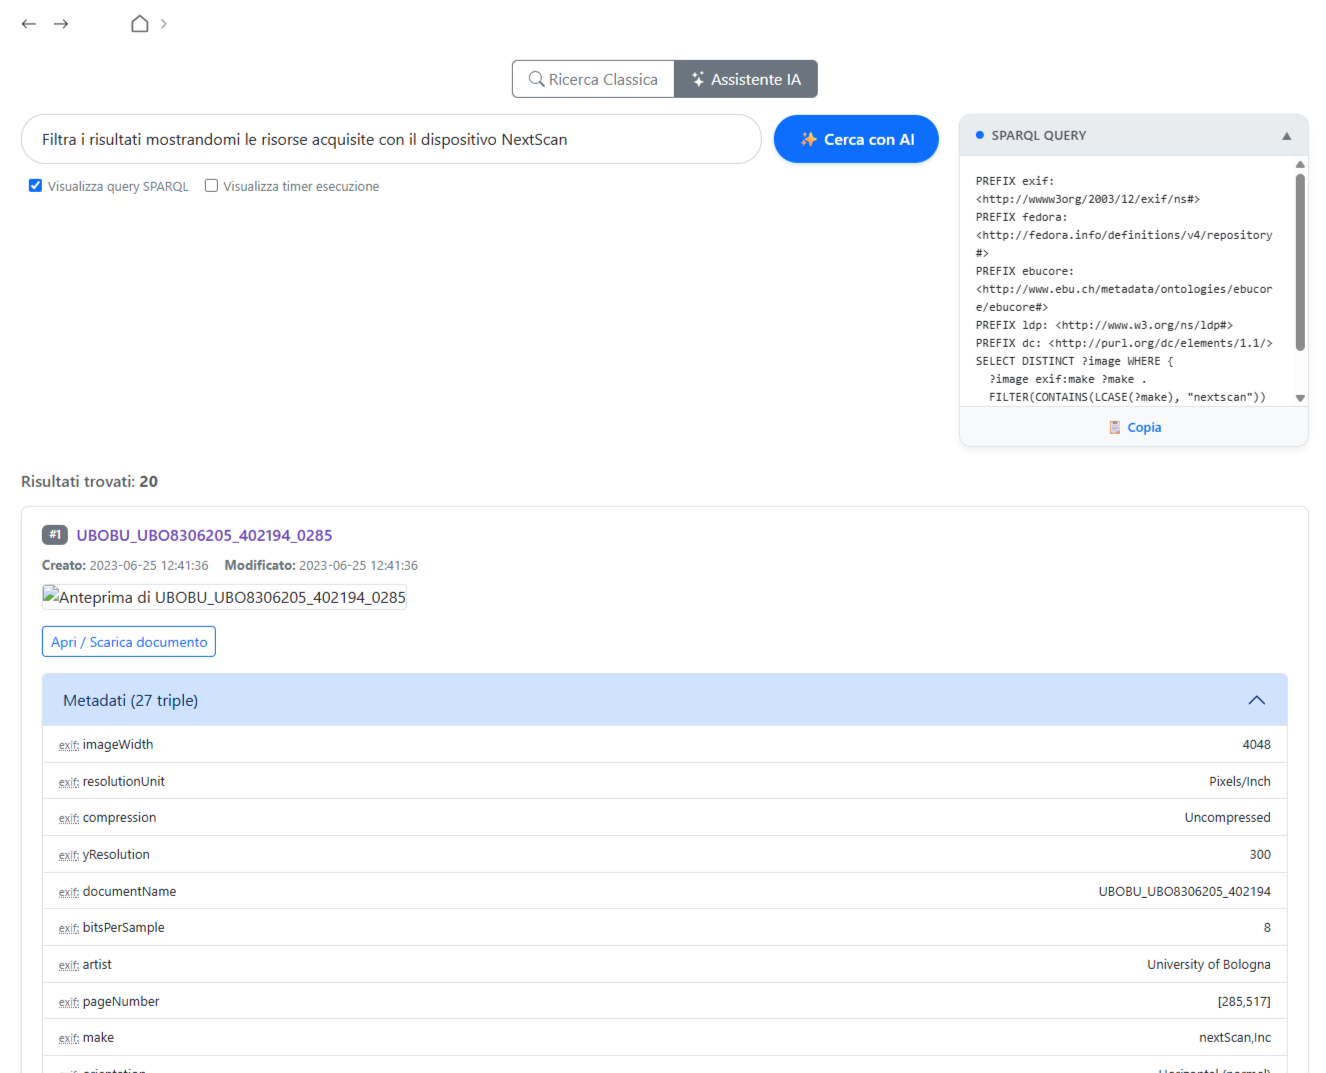
\includegraphics[width=0.9\textwidth]{../img/caso_uso_1.png}
            \caption{Caso d'uso 1: Estrazione delle risorse corrispondenti al dispositivo NextScan.}\label{fig:caso_uso1}
        \end{figure}
        \vfill

        \textbf{Risoluzione del problema}: Oltre a delegare all'LLM l'onere della traduzione del linguaggio naturale nel predicato corretto (\code{exif:make}), questo scenario dimostra la resilienza dell'architettura. 

    \subsection{Caso d'uso 2: disambiguazione semantica dell'autore}\label{subsec:cu2}
        \textbf{Attore}: un responsabile di un progetto di digitalizzazione o ricercatore interessato alla provenienza materiale dello scatto.\\
        \textbf{Input testuale}: 
        \begin{center}
            \code{``Filtra le risorse mostrandomi i file in cui}
            \code{l'autore dello scatto è University''}
        \end{center}
        \vspace{0.5em}

        \begin{lstlisting}[language=sparql, caption=Caso d'uso 2: Query SPARQL per disambiguazione autore, basicstyle=\ttfamily\scriptsize, breaklines=true]
  PREFIX exif: <http://wwww3org/2003/12/exif/ns#>
  PREFIX fedora: <http://fedora.info/definitions/v4/repository#>
  PREFIX ebucore: <http://www.ebu.ch/metadata/ontologies/ebucore/ebucore#>
  PREFIX ldp: <http://www.w3.org/ns/ldp#>
  PREFIX dc: <http://purl.org/dc/elements/1.1/>
  SELECT DISTINCT ?image WHERE {
      ?image exif:artist ?artist .
      FILTER(CONTAINS(LCASE(?artist), "university"))
  }
  LIMIT 20\end{lstlisting}

        \begin{figure}[H]
            \centering
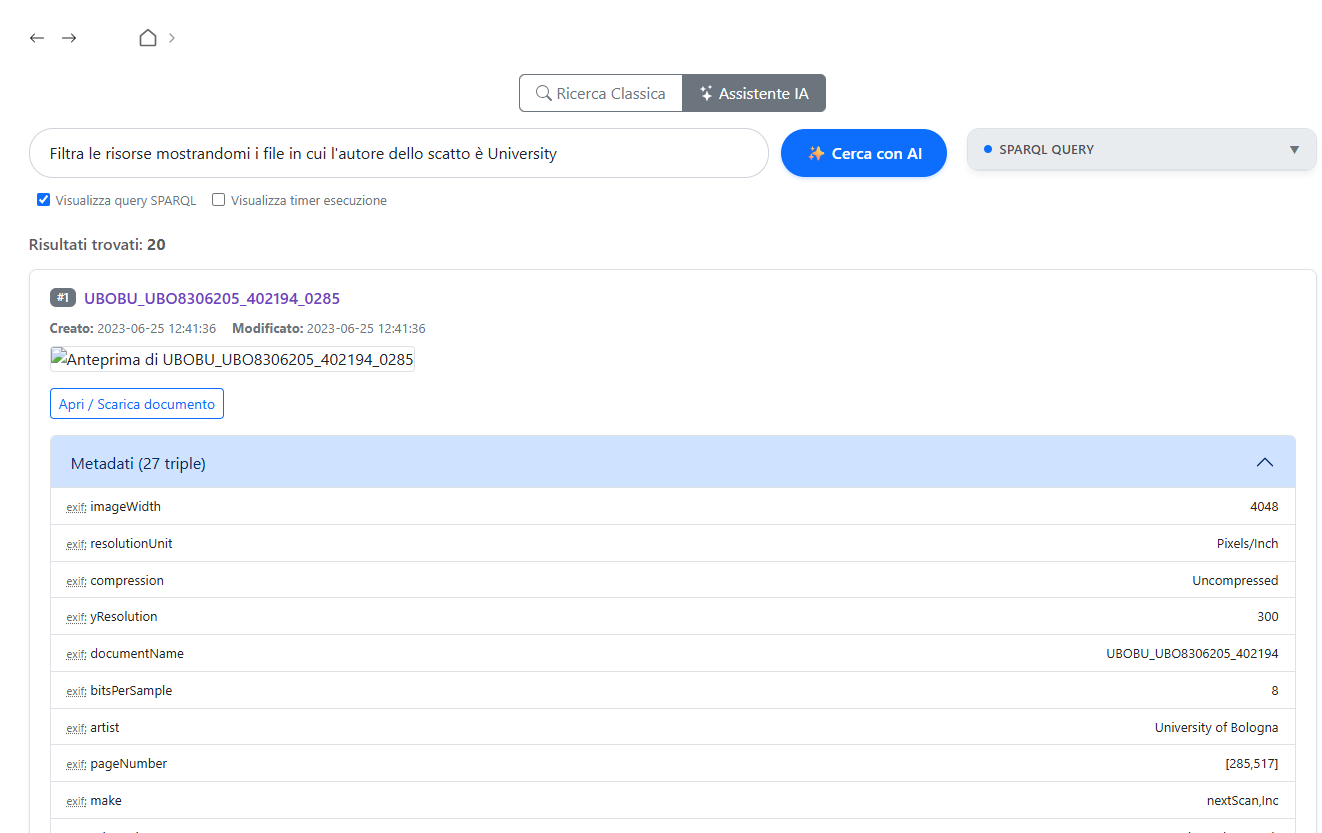
\includegraphics[width=0.9\textwidth]{../img/caso_uso_2.png} 
            \caption{Caso d'uso 2: Disambiguazione semantica dell'autore e visualizzazione dei risultati.}\label{fig:caso_uso2}
        \end{figure}

        \textbf{Risoluzione del problema}: Questo scenario evidenzia la capacità dell'LLM di operare una corretta disambiguazione semantica. Il modello comprende l'intento dell'utente distinguendo l'autore materiale dello scatto (\code{exif:artist}) dall'utente responsabile del caricamento nel Data Vault (\code{fedora:createdBy}).

    \newpage
        \subsection{Caso d'uso 3: ricerca multi-criterio con filtro temporale}\label{subsec:cu3}
        \textbf{Attore}: un ricercatore che vuole analizzare la produzione digitale filtrandola all'interno di un preciso arco temporale.\\
        \textbf{Input testuale}: 
        \begin{center}
            \code{``Mostrami tutte le risorse comprese tra l'anno 2023 e il 2026''}
        \end{center}
        \vspace{0.5em}

        \begin{lstlisting}[language=sparql, caption=Caso d'uso 3: Query SPARQL per ricerca con filtro temporale, basicstyle=\ttfamily\scriptsize, breaklines=true]
  PREFIX exif: <http://wwww3org/2003/12/exif/ns#>
  PREFIX ebucore: <http://www.ebu.ch/metadata/ontologies/ebucore/ebucore#>   
  PREFIX fedora: <http://fedora.info/definitions/v4/repository#>
  PREFIX ldp: <http://www.w3.org/ns/ldp#>
  PREFIX dc: <http://purl.org/dc/elements/1.1/>
  SELECT DISTINCT ?image WHERE {
      ?image exif:dateTime ?date .
      FILTER(STR(?date) >= "2023" && STR(?date) <= "2026")
  }
  LIMIT 20\end{lstlisting}

        \begin{figure}[H]
            \centering
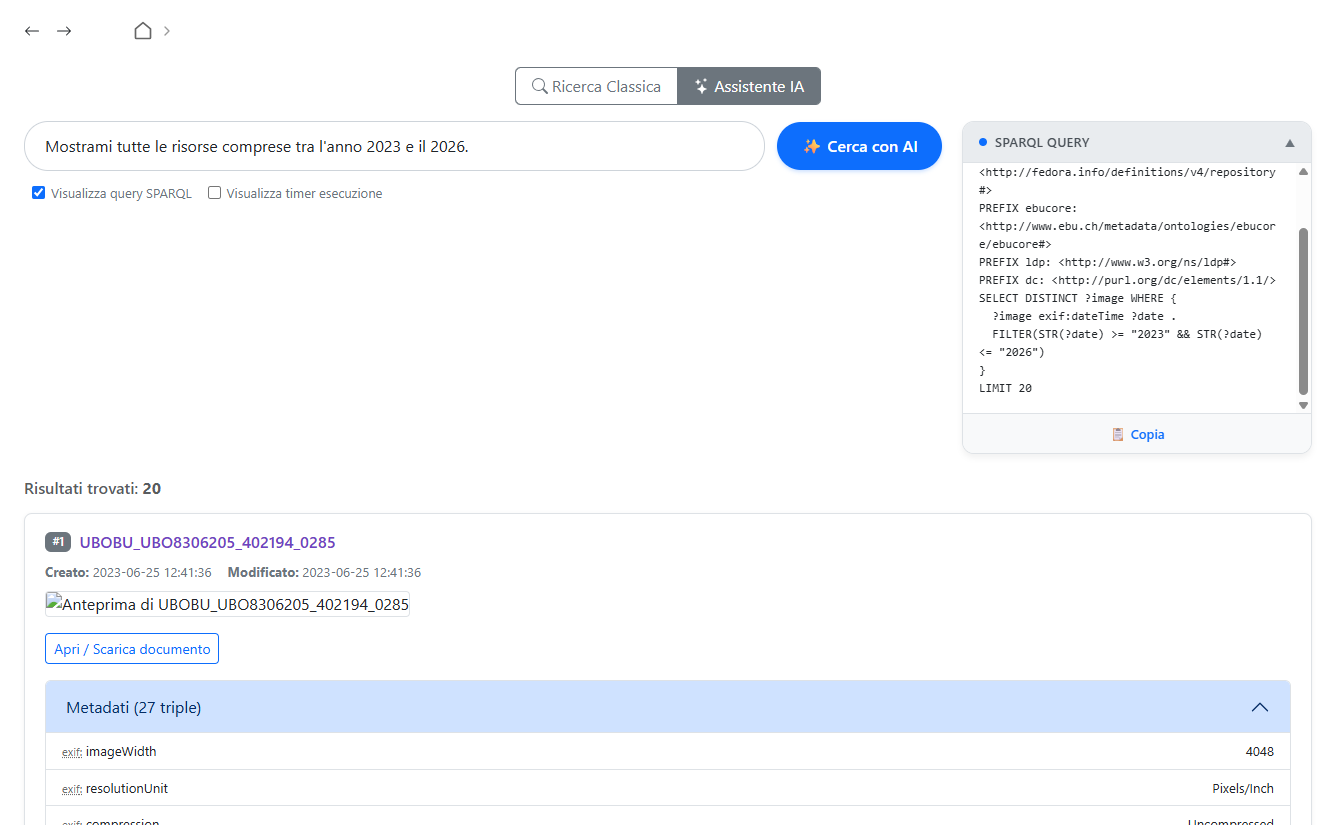
\includegraphics[width=0.9\textwidth]{../img/caso_uso_3.png} 
            \caption{Caso d'uso 3: Applicazione logica del range temporale ed estrazione delle immagini.}\label{fig:caso_uso3}
        \end{figure}

        \textbf{Risoluzione del problema}: L'estrazione basata su range temporali richiede una sintassi SPARQL rigorosa e insidiosa per un utente non tecnico. Il sistema individua automaticamente il predicato \code{exif:dateTime} e costruisce i costrutti logici di comparazione testuale (\code{>=} e \code{<=}).
    \newpage
    \section{Conclusioni del capitolo}\label{sec:conclusioni_cap3}
        In questo capitolo abbiamo presentato il prototipo e la sua interfaccia, rispondendo attivamente alle criticità sollevate nel \cref{chap:contesto}:
        \begin{enumerate}
            \item Il problema della \textbf{``scatola vuota''} e la paralisi decisionale (Legge di Hick) sono stati superati adottando un'interfaccia basata unicamente sull'input testuale naturale.
            \item L'obbligo di conoscere schemi complessi (es.\ prefissi EXIF o Dublin Core) è stato demandato al backend, azzerando il carico cognitivo per l'utente finale.
        \item La rigidità formale di SPARQL è stata assorbita dall'LLM, che agisce come mediatore invisibile.
    \end{enumerate}

    Il \cref{chap:implementazione} approfondirà il dietro le quinte tecnologico: la struttura del backend, l'ottimizzazione del proxy Vite e il delicato processo di fine-tuning del modello linguistico. 
\chapter{Architettura e dettagli implementativi}\label{chap:implementazione}

\section{Introduzione al capitolo}\label{sec:intro_cap4}

In questo capitolo viene illustrata nel dettaglio l'architettura tecnica e le scelte implementative che costituiscono il motore dell'LLM Query Builder. Se il \cref{chap:prototipo} ha descritto il sistema dal punto di vista dell'utente finale focalizzandosi sulla transizione da domanda naturale a risultati navigabili, in questo capitolo verranno analizzati i componenti software, lo stack tecnologico e le metodologie di addestramento che rendono possibile tale comportamento.

Il capitolo segue il flusso logico della costruzione del sistema: si parte dall'infrastruttura di base e dalle scelte tecnologiche complessive (\cref{sec:stack}), passando alla pipeline di fine-tuning del modello (\cref{sec:finetuning}), quindi si analizza l'architettura del backend e l'integrazione con il frontend (\cref{sec:backend}), per concludere con il formato e la struttura del dataset di addestramento (\cref{sec:dataset}).

\section{Stack tecnologico: Fedora e Blazegraph}\label{sec:stack}
  \begin{figure}[htbp]
    \centering
\resizebox{\textwidth}{!}{
      \begin{tikzpicture}[
node distance=1.6cm and 2.6cm, 
        box/.style={rectangle, draw=black, thick, rounded corners, minimum width=3.2cm, minimum height=1.4cm, align=center, fill=blue!5, font=\small},
        db/.style={cylinder, draw=black, thick, aspect=0.25, shape border rotate=90, minimum width=3.2cm, minimum height=1.4cm, align=center, fill=green!5, font=\small},
        arrow/.style={-Latex, thick}
      ]

\node[box] (frontend) {\textbf{Browser Frontend} \\ (React)};
      \node[box, right=of frontend] (backend) {\textbf{FastAPI Backend} \\ (Inference Engine)};
      \node[box, right=of backend] (llm) {\textbf{LLM Model} \\ (Phi-3-mini)};
      \node[db, below=of backend] (blazegraph) {\textbf{Blazegraph} \\ (Triplestore)};



\draw[arrow] ([yshift=2.5mm]frontend.east) -- node[above, font=\scriptsize, midway, align=center] {HTTP \\ POST} ([yshift=2.5mm]backend.west);
      \draw[arrow] ([yshift=-2.5mm]backend.west) -- node[below, font=\scriptsize, midway, align=center] {JSON \\ (Risultati)} ([yshift=-2.5mm]frontend.east);

\draw[arrow] ([yshift=2.5mm]backend.east) -- node[above, font=\scriptsize, midway, align=center] {Prompt} ([yshift=2.5mm]llm.west);
      \draw[arrow] ([yshift=-2.5mm]llm.west) -- node[below, font=\scriptsize, midway, align=center] {Query \\ SPARQL} ([yshift=-2.5mm]backend.east);

\draw[arrow] (backend.255) -- node[left, font=\scriptsize, midway] {SPARQL} (blazegraph.105);
      \draw[arrow] (blazegraph.75) -- node[right, font=\scriptsize, midway] {RDF Bindings} (backend.285);

      \end{tikzpicture}
    }
    \caption{Architettura logica e flusso di comunicazione del sistema. 
}\label{fig:arch_logica}
  \end{figure}

  L'infrastruttura dati su cui si appoggia l'LLM Query Builder è costituita da Fedora e Blazegraph. 
  Blazegraph, in particolare, opera come triplestore ad alte prestazioni per il Datavault, fornendo l'endpoint SPARQL interrogato dal nostro sistema.
  Il lavoro è consistito nel creare un layer intermedio capace di dialogare fluidamente con Blazegraph, astraendo la sintassi del linguaggio SPARQL dall'interfaccia esposta al ricercatore.

  \subsection{I tre layer del sistema}\label{subsec:tre_layer}
    A livello logico, il sistema suddivide il flusso di lavoro in tre layer:
    \begin{itemize}
      \item \textbf{Presentazione (Datavault Browser)}: applicazione React con due barre di ricerca testuale, una per una ricerca google-like \code{<SearchField/>} e una per una ricerca avanzata con il tool \code{<LLMSearchBar/>} selezionabili da un bottone centrato sopra di esse.
      In modalità ``Assistente IA'', è possibile la visualizzazione della query SPARQL generata per utenti più esperti. Raccoglie l'input testuale dell'utente e lo invia al backend.
      \item \textbf{Applicativo (LLM Query Builder backend, FastAPI)}: il ``cervello'' del sistema che riceve la domanda naturale, dirige il flusso:
      
      \begin{center}
        \begin{tikzpicture}[
          node distance=0.8cm,
          stepbox/.style={rectangle, draw=black, thick, rounded corners, minimum height=0.9cm, inner sep=6pt, align=center, fill=blue!5, font=\small},
          arrow/.style={-Latex, thick}
        ]
          \node[stepbox] (prompt) {Costruzione\\del prompt};
          \node[stepbox, right=of prompt] (inferenza) {Inferenza\\LLM};
          \node[stepbox, right=of inferenza] (validazione) {Validazione};
          \node[stepbox, right=of validazione] (esecuzione) {Esecuzione\\SPARQL};
          \draw[arrow] (prompt) -- (inferenza);
          \draw[arrow] (inferenza) -- (validazione);
          \draw[arrow] (validazione) -- (esecuzione);
        \end{tikzpicture}
      \end{center}

      e gestisce gli errori (query malformate, allucinazioni, timeout, richieste out-of-domain) e restituisce risultati strutturati al frontend.
      \item \textbf{LDati (Datavault / Blazegraph)}: immagazzina i milioni di triple RDF del Datavault, esegue la query SPARQL ricevuta dal backend e ne restituisce i risultati grezzi.
    \end{itemize}

  \subsection{Il flusso end-to-end di una richiesta}\label{subsec:flusso_e2e}

    Una richiesta tipica attraversa il sistema secondo i seguenti passi:

    \begin{enumerate}
      \item L'utente digita una domanda in linguaggio naturale (es.\ ``Mostrami le immagini scansionate con una Nikon nel 2022'') nella barra di ricerca del frontend.
      \item Il frontend invia un \code{HTTP POST} al backend con il testo della domanda.
      \item Il backend costruisce il prompt completo (system prompt con le regole di generazione + domanda dell'utente, si veda \cref{subsec:regole}) e lo sottopone al modello LLM.\@
      \item Il modello genera una query SPARQL (o un JSON di errore, se la richiesta è fuori dominio).
      \item Il backend ripulisce e valida l'output (si veda il ``sanitizzatore'', \cref{subsec:fastapi}).
      \item Se valida, la query viene eseguita su Blazegraph.
      \item I risultati vengono trasformati in struttura ad albero e restituiti al frontend, che li visualizza in forma navigabile.
    \end{enumerate}

  \subsection{Scelte tecnologiche principali}\label{subsec:scelte_tech}
    Il sistema combina le seguenti tecnologie, ciascuna scelta per ragioni specifiche legate ai vincoli del progetto:

    \begin{itemize}
      \item \textbf{React} (frontend): per la parte di presentazione, già descritta funzionalmente nel \cref{chap:prototipo}.
      \item \textbf{FastAPI} (backend): scelto per la type safety offerta da Pydantic, la documentazione automatica, le performance asincrone e la facilità di integrazione diretta con PyTorch/Transformers per servire il modello.
      \item \textbf{Phi-3-mini} (modello LLM base): dimensione contenuta (3.8 miliardi di parametri) che rende fattibile il fine-tuning mantenendo buone performance di base su compiti di generazione strutturata.
      \item \textbf{Unsloth + LoRA} (fine-tuning): Unsloth velocizza il fine-tuning e riduce il consumo di memoria; LoRA (Low-Rank Adaptation) permette di adattare il modello aggiornando solo un numero ridotto di parametri, evitando i costi proibitivi del full fine-tuning.
      \item \textbf{Blazegraph} (triplestore): tecnologia già in uso presso DH.ARC per il Datavault, con supporto nativo a SPARQL 1.1 e scalabilità fino a centinaia di milioni di triple.
    \end{itemize}



\section{Pipeline di fine-tuning dell'LLM}\label{sec:finetuning}
  Per ottenere traduzioni accurate dal linguaggio naturale a SPARQL, l'utilizzo di un LLM generico si è rivelato insufficiente: un modello addestrato su testo web conosce SPARQL in linea di principio, ma non è ottimizzato per generare query corrette per lo specifico schema del Datavault, rischiando di allucinare predicati inesistenti o di non comprendere le particolarità dell'ontologia reale. Si è resa quindi necessaria una fase di \textit{domain adaptation} tramite fine-tuning.

  \subsection{Dataset generativo e schema SPARQL}\label{subsec:dataset_gen}
    L'addestramento è stato basato su un dataset generativo, prodotto tramite lo script \code{genera\_dataset.py} secondo un approccio a \textbf{template parametrici}: per ciascuna categoria di query viene definita una funzione Python che, dati alcuni parametri (un anno, un nome di dispositivo, un formato file, ecc.), restituisce la query SPARQL corrispondente già popolata con quei valori. 
    La domanda in linguaggio naturale che accompagna ciascuna query viene generata in parallelo variando lessico e struttura della frase, in modo da esporre il modello a una pluralità di formulazioni per lo stesso intento.

    \subsubsection{Il ciclo di generazione}
      Il cuore del generatore è il ciclo di costruzione del dataset, riportato (in forma semplificata) di seguito:

      \begin{lstlisting}[language=python, caption=Struttura del ciclo di generazione del dataset]
def crea_dataset_massivo(target: int = 10000):
  # ... inizializzazione contatori ...
  tipi_sparql = list(range(1, 14))

  while conteggio < target:
    # Iniezione controllata di esempi Fuori Dominio
    forza_ood = (ood_count < ood_target) and (
      sparql_count >= sparql_target or random.random() < 0.15
    )
    if forza_ood:
      frase = random.choice(out_of_domain)
      query = '{"error": "OUT_OF_DOMAIN"}'
      ood_count += 1
    else:
      # Estrazione di una categoria e popolamento del template
      tipo = random.choice(tipi_sparql)
      if tipo == 1:
        ...  # popolamento template categoria 1
      elif tipo == 2:
        ...  # popolamento template categoria 2
      # [...]
      else:  # tipo == 13
        ...  # popolamento template categoria 13

    # Salvataggio in formato JSONL pronto per il fine-tuning,
    # con lo stesso system prompt usato in inferenza
    riga_dataset = {
      "messages": [
        {"role": "system",  "content": SYSTEM_PROMPT},
        {"role": "user",    "content": frase},
        {"role": "assistant", "content": query},
      ]
    }
\end{lstlisting}

Questa struttura garantisce due proprietà desiderabili per il dataset: una distribuzione controllata tra le diverse categorie di query (evitando lo sbilanciamento verso le categorie più semplici da generare), e un'iniezione mirata di esempi out-of-domain in proporzione fissa (circa il 10\% del totale), necessaria affinché il modello impari a riconoscere e rifiutare richieste estranee al dominio del Datavault senza che questo comportamento venga sotto-rappresentato nel training.
Inoltre, l'approccio generativo ha man mano permesso di raffinare gli esempi, correggendo a monte gli errori sistematici nella gestione dei prefissi ontologici e dei metadati emersi durante le prime fasi di test del modello.

\subsubsection{Le 13 categorie di query SPARQL (+1 Out-of-Domain)}

La versione finale del generatore comprende 13 funzioni template, ciascuna corrispondente a un intento di ricerca distinto. Le funzioni sono state progettate per coprire lo spettro delle interrogazioni tipiche del dominio umanistico, più la gestione separata delle query fuori dominio:

\begin{table}[htbp]
    \centering
    \begin{tabularx}{\textwidth}{cl>{\raggedright\arraybackslash}X}
        \toprule
        \textbf{\#} & \textbf{Funzione} & \textbf{Categoria} \\
        \midrule
        1  & \code{query\_autore\_anno}    & Ricerca combinata: autore dello scatto + anno \\
        2  & \code{query\_dispositivo}     & Ricerca per dispositivo di acquisizione (\code{exif:make}) \\
        3  & \code{query\_anno}            & Ricerca generica per anno \\
        4  & \code{GOLDEN\_QUERY\_LIBERA}  & Richiesta dell'intero archivio (``mostrami tutto'') \\
        5  & \code{query\_container}       & Ricerca in una cartella/container (\code{ldp:contains+}) \\
        6  & \code{query\_testo}           & Ricerca full-text su nome file (\code{ebucore:filename}) \\
        7  & \code{query\_formato}         & Filtro per formato/MIME type (es.\ \code{image/jpeg}) \\
        8  & \code{query\_data\_esatta}    & Ricerca per data precisa (anno, mese, giorno) \\
        9  & \code{query\_intervallo\_anni} & Ricerca per intervallo temporale (range di anni) \\
        10 & \code{query\_not\_anno}       & Negazione: esclusione di un anno specifico \\
        11 & \code{query\_or\_formati}     & OR logico tra due formati file \\
        12 & \code{query\_limite\_custom}  & Paginazione: restituzione degli ultimi N file \\
        13 & \code{query\_uploader}        & Ricerca per autore del caricamento (\code{fedora:createdBy}) \\
        \midrule
        --- & \textit{(separato)} & Out-of-Domain: richieste estranee al dominio ($\sim$10\% del dataset) \\
        \bottomrule
    \end{tabularx}
    \caption{Le 13 categorie di query SPARQL generate da \code{genera\_dataset.py}, più la categoria Out-of-Domain gestita a parte nel ciclo di generazione.}\label{tab:categorie_template}
\end{table}
Si noti come le categorie 1 e 13 condividano lo stesso intento superficiale (``ricerca per autore'') ma si distinguano per il predicato RDF target (\code{exif:artist} per l'autore dello scatto, \code{fedora:createdBy} per chi ha effettuato il caricamento): questa distinzione, esplicitata anche nella Regola 2 del system prompt (\cref{subsec:regole}), rappresenta uno degli edge case linguistici più rilevanti affrontati nella progettazione del dataset.

\subsubsection{Edge case e bug risolti durante la generazione}\label{subsec:edge_cases_generazione}

Durante la fase di validazione, l'analisi delle query fallite aveva evidenziato un tasso di errore significativo dovuto a una scorretta generazione della sintassi SPARQL, in particolare a causa di un'errata gestione dei prefissi dei metadati. Per risolvere la problematica in modo strutturale, si è proceduto a raffinare gli esempi all'interno del dataset di addestramento, correggendo esplicitamente il modo in cui il modello mappa e dichiara i prefissi ontologici, e gestendo puntualmente i \textit{type-mismatch} tra proprietà testuali e numeriche. Nello specifico, gli edge case principali risolti sono stati:

\begin{itemize}
  \item \textbf{Type mismatch su date}: il formato del filtro temporale era inizialmente incoerente con \code{xsd:dateTime} --- risolto normalizzando il formato nei template e, come descritto nella Regola 6 del system prompt, imponendo il confronto tramite \code{STR()} anziché tramite tipi di dato tipizzati.
  \item \textbf{Case-sensitivity nei filtri di negazione} --- risolto normalizzando i predicati nel template generatore.
  \item \textbf{Generazione di date calendarialmente non valide} (es.\ 30 febbraio) --- risolto validando le date generate con la libreria Python \code{datetime}.
  \item \textbf{Ambiguità del separatore nelle date EXIF} (\code{:} vs \code{-}) --- risolto unificando il formato nel dataset.
\end{itemize}

\subsubsection{Schema RDF reale e un bug di produzione nel namespace EXIF}\label{subsec:bug_exif_namespace}


\begin{table}[h]
  \centering
  \renewcommand{\arraystretch}{1.2}
  \begin{tabularx}{\textwidth}{@{} p{5cm} r >{\raggedright\arraybackslash}X @{}}
    \toprule
    Predicato & Frequenza & Significato \\
    \midrule
    \code{rdf:type}                      & 2.707.278 & Tipizzazione della risorsa \\
    \code{ldp:contains}                  & 676.186   & Rel.\ di contenimento container $\to$ risorsa \\
    \code{ebucore:filename}              & 674.985   & Nome del file \\
    \code{ebucore:hasMimeType}           & 674.985   & Tipo MIME della risorsa \\
    \code{premis:hasSize}                & 674.985   & Dimensione del file \\
    \code{exif:dateTime}                 & 674.959   & Data/ora di acquisizione \\
    \code{exif:make / exif:model}        & 674.959   & Dispositivo di acquisizione \\
    \code{exif:imageWidth}               & 672.607   & Dimensioni in pixel \\
    \code{dc:title}                      & 1.196     & Titolo (solo sui container) \\
    \bottomrule
  \end{tabularx}
  \caption{Predicati principali dello schema RDF del Datavault, con frequenza osservata}\label{tab:schema_predicati}
\end{table}

Durante l'analisi della distribuzione dei predicati nel triplestore di produzione è emerso che il namespace EXIF effettivamente presente in Blazegraph è malformato: \url{http://wwww3org/2003/12/exif/ns#}, anziché lo standard \url{http://www.w3.org/2003/12/exif/ns#} (mancano i due punti e il prefisso \code{www.} corretto). Il bug è stato confermato eseguendo una query SPARQL di verifica diretta sull'endpoint:

\begin{lstlisting}[language=sparql, caption=Query di verifica del namespace EXIF reale]
SELECT DISTINCT ?p WHERE {
  ?s ?p ?o .
  FILTER(CONTAINS(STR(?p), "exif"))
} LIMIT 5
\end{lstlisting}

\paragraph{Impatto del bug.} Questo mismatch ha un impatto sistemico: qualunque query SPARQL generata utilizzando il namespace EXIF \textit{canonico} (quello atteso da un modello addestrato su conoscenza generale o su un dataset che rispetti lo standard W3C) restituisce sistematicamente zero risultati per tutti i predicati EXIF, indipendentemente dalla correttezza logica della query stessa. Poiché i predicati EXIF coprono la quasi totalità delle risorse del Datavault, questo bug avrebbe potuto compromettere la quasi totalità delle interrogazioni utili del sistema.

\paragraph{Soluzione adottata: allineamento al dato reale, non correzione.} A differenza di un approccio ``correttivo'' (normalizzare il namespace malformato a quello standard prima dell'esecuzione della query), la soluzione adottata è stata l'\textbf{allineamento sistematico al namespace reale}, poiché il typo è presente fisicamente nei dati e non è modificabile lato Datavault. Qualunque normalizzazione verso il namespace standard avrebbe prodotto query sintatticamente corrette ma semanticamente vuote. La soluzione è stata applicata in due punti della pipeline:

\begin{enumerate}
  \item \textbf{Generazione del dataset di training} (\code{genera\_dataset.py}): il prefisso malformato è stato hardcoded esplicitamente tra i prefissi fissi usati per generare gli esempi di training, con un commento esplicito a documentazione della scelta:
\begin{lstlisting}[language=python, caption=Prefissi hardcoded nel generatore del dataset]
# Il prefisso exif MANTIENE il typo "wwww3org" per matchare il tuo DB reale
PREFISSI = (
  "PREFIX exif: <http://wwww3org/2003/12/exif/ns#>\n"
  # ...
)
\end{lstlisting}
  In questo modo il modello, durante il fine-tuning, apprende direttamente a generare query con il namespace realmente presente in produzione.
  \item \textbf{Backend di inferenza} (\code{main.py}): per garantire robustezza anche nel caso in cui il modello generi (o allucini) un prefisso diverso da quello atteso, il backend rimuove qualunque blocco di prefissi generato dall'LLM e re-inietta forzatamente un blocco di prefissi hardcoded, contenente anch'esso il namespace malformato (si veda \cref{subsec:fastapi} per il dettaglio del sanitizzatore).
\end{enumerate}

\paragraph{Considerazioni.} Questa soluzione, per quanto pragmatica, espone una fragilità intrinseca dell'approccio: il sistema è ora \textit{accoppiato} a un errore presente nei dati di produzione. Se in futuro il Datavault venisse corretto o migrato verso un namespace EXIF standard, sia il dataset di training sia il backend richiederebbero un aggiornamento sincronizzato per evitare di reintrodurre lo stesso problema in forma invertita. Questo aspetto viene ripreso come punto di attenzione nel \cref{chap:conclusioni} (sviluppi futuri) e il suo impatto sulle metriche di valutazione è discusso nel \cref{chap:valutazione}.



\newpage

\subsection{Configurazione dell'addestramento con Unsloth}\label{subsec:unsloth}
    Per ottimizzare i tempi di addestramento e ridurre l'impronta in memoria VRAM, la pipeline è stata implementata avvalendosi della libreria Unsloth, che fornisce un'integrazione nativa e ottimizzata per il fine-tuning con LoRA (Low-Rank Adaptation) su modelli come Phi-3.

    \subsubsection{L'algoritmo LoRA}
        LoRA evita i costi proibitivi di un full fine-tuning (che richiederebbe risorse GPU non disponibili sull'hardware consumer usato per il training) congelando i pesi originali del modello e introducendo, per ciascuna matrice di pesi $W$ presa di mira, un aggiornamento di basso rango: $W' = W + \frac{\alpha}{r}BA$ dove $B \in \mathbb{R}^{d \times r}$ e $A \in \mathbb{R}^{r \times k}$, con il rank $r \ll \min(d,k)$. Durante il training vengono aggiornate solamente le matrici $A$ e $B$, riducendo il numero di parametri allenabili rispetto ai miliardi di parametri del modello completo.\\
        Nel nostro caso $r = 16 = \alpha$ (quindi $\alpha/r = 1$, nessuno scaling aggiuntivo dell'aggiornamento), applicato sia ai proiettori di attention (\code{q/k/v/o\_proj}) sia ai proiettori del blocco feed-forward (\code{gate/up/down\_proj}): una scelta più estensiva rispetto a una LoRA limitata alla sola attention, che aumenta la capacità del modello di adattarsi al vocabolario specifico del dominio (predicati RDF, sintassi SPARQL) a fronte di un numero di parametri allenabili comunque contenuto grazie al rank ridotto.

\subsubsection{Iperparametri utilizzati}\label{subsec:hyperparams}

\begin{table}[htbp]
  \centering
  \renewcommand{\arraystretch}{1.2}
  \begin{tabularx}{\textwidth}{@{} p{6.5cm} >{\raggedright\arraybackslash}X @{}} \toprule
  \textbf{Parametro} & \textbf{Valore} \\
  \midrule
  \textbf{Modello base} & \code{unsloth/Phi-3-mini-4k-instruct} \\
  \midrule
  \multicolumn{2}{@{}l}{\textbf{Configurazione LoRA}} \\
  \addlinespace
  \quad LoRA rank ($r$) & 16 \\
  \quad LoRA alpha & 16 \\
  \quad LoRA dropout & 0 \\
  \quad Target modules & \code{q\_proj, k\_proj, v\_proj, o\_proj,} \newline \code{gate\_proj, up\_proj, down\_proj} \\
  \quad Bias & \code{none} \\
  \quad Gradient checkpointing & \code{True} \\
  \quad Random state & 3407 \\
  \bottomrule
  \end{tabularx}
  \caption{Iperparametri di fine-tuning LoRA (1/2): modello base e configurazione dell'adapter LoRA, configurato tramite Unsloth.}\label{tab:hyperparams_lora}
\end{table}
\newpage
\begin{table}[ht]
  \centering
  \renewcommand{\arraystretch}{1.2}
  \begin{tabularx}{\textwidth}{@{} p{6.5cm} >{\raggedright\arraybackslash}X @{}}
  \toprule
  \textbf{Parametro} & \textbf{Valore} \\
  \midrule
  \quad Batch size (per device) & 1 \\
  \quad Gradient accumulation steps & 8 \\
  \quad Batch size effettivo & 8 (1 $\times$ 8) \\
  \quad Warmup steps & 10 \\
  \quad Epochs & 1 \\
  \quad Learning rate & \code{2e-4} \\
  \quad Optimizer & \code{adamw\_8bit} \\
  \quad Weight decay & 0.01 \\
  \quad LR scheduler & \code{linear} \\
  \quad Seed & 3407 \\
  \quad fp16 / bf16 & \code{False} / \code{False} \\
  \quad Packing & \code{False} \\
  \quad Dataset num proc & 2 \\
  \quad Max sequence length & 1024 token \\
  \quad Step totali eseguiti & 1188 \\
  \quad Loss finale & 0.010 \\
  \bottomrule
  \end{tabularx}
  \caption{Iperparametri di fine-tuning LoRA (2/2): configurazione del training tramite \code{SFTTrainer} (libreria TRL).}\label{tab:hyperparams_training}
\end{table}

Il valore di \code{max\_seq\_length} è stato fissato a 1024 token: sufficiente a contenere il system prompt (regole di generazione), la domanda dell'utente in linguaggio naturale, e la query SPARQL attesa, mantenendo comunque un footprint di memoria contenuto durante il training su GPU con VRAM limitata.
 
Il codice di configurazione effettivamente utilizzato è riportato di seguito. Il primo passo è il caricamento del modello base tramite Unsloth:

\vfill
 
\begin{lstlisting}[language=python, caption=Caricamento del modello base]
import torch
from unsloth import FastLanguageModel
 
max_seq_length = 1024
dtype = torch.float16
load_in_4bit = False
 
model, tokenizer = FastLanguageModel.from_pretrained(
    model_name = "unsloth/Phi-3-mini-4k-instruct",
    max_seq_length = max_seq_length,
    dtype = dtype,
    load_in_4bit = load_in_4bit,
)
\end{lstlisting}
 
Da notare che il modello viene caricato in precisione \code{float16} e senza quantizzazione a 4 bit: questo è distinto dai flag \code{fp16}/\code{bf16} del \code{SFTTrainer} (entrambi \code{False}), che controllano invece l'uso di \textit{mixed precision training} (autocast durante il calcolo del gradiente) e non la precisione nativa dei pesi del modello.
 
Segue la configurazione dell'adapter LoRA e del training vero e proprio:
 
\begin{lstlisting}[language=python, caption=Configurazione dell'adapter LoRA tramite Unsloth]
model = FastLanguageModel.get_peft_model(
    model,
    r = 16,
    target_modules = ["q_proj", "k_proj", "v_proj", "o_proj",
                       "gate_proj", "up_proj", "down_proj"],
    lora_alpha = 16, lora_dropout = 0,
    bias = "none",   use_gradient_checkpointing = True,
    random_state = 3407,
)
\end{lstlisting}
 
\begin{lstlisting}[language=python, caption=Configurazione del training tramite SFTTrainer (libreria TRL)]
from trl import SFTTrainer, SFTConfig
trainer = SFTTrainer(
    model = model, tokenizer = tokenizer,
    train_dataset = train_dataset,
    eval_dataset = eval_dataset,
    args = SFTConfig(
        per_device_train_batch_size = 1,
        gradient_accumulation_steps = 8,
        warmup_steps = 10,
        num_train_epochs = 1,
        learning_rate = 2e-4,
        fp16 = False, bf16 = False,
        logging_steps = 10,
        eval_strategy = "steps",
        eval_steps = 50,
        save_strategy = "steps",
        save_steps = 100,
        save_total_limit = 2,
        report_to = "none",
        optim = "adamw_8bit",
        weight_decay = 0.01,
        lr_scheduler_type = "linear",
        seed = 3407,
        output_dir = "outputs",
        dataset_text_field = "text",
        max_seq_length = max_seq_length,
        dataset_num_proc = 2,
        packing = False,
    ),
)
\end{lstlisting}


\section{Architettura del backend e integrazione frontend}\label{sec:backend}


\subsection{Inference engine (FastAPI)}\label{subsec:fastapi}
Il coordinamento delle richieste è affidato a un backend sviluppato in Python tramite FastAPI.\@
L'inference engine è stato calibrato per garantire la consistenza del \textit{system prompt} a ogni invocazione, vincolando il modello a mantenere il ruolo di traduttore tecnico.
È stata posta particolare attenzione alla corretta generazione del token EOS (\textit{End Of Sentence}), fondamentale per troncare l'output del modello ed evitare allucinazioni aggiuntive in coda alla query SPARQL.\@

  \subsubsection{Caricamento del modello e fusione dell'adapter LoRA}

  \begin{sloppypar}
  A differenza del notebook di training (dove il modello viene caricato tramite \code{FastLanguageModel} di Unsloth), il backend di inferenza carica il modello tramite le primitive standard di Hugging Face Transformers e PEFT, eseguendo il caricamento una sola volta all'avvio del server e non ad ogni richiesta, per evitare il costo proibitivo di ricaricare e fondere il modello a ogni chiamata:
  \end{sloppypar}

  \begin{lstlisting}[language=python, caption=Caricamento e fusione dell'adapter LoRA all'avvio del server FastAPI]
@app.on_event("startup")
async def load_model():
  global model, tokenizer
  print("Inizializzazione del motore LLM...")

  tokenizer = AutoTokenizer.from_pretrained(ADAPTER_PATH)

  # Usiamo la versione base per evitare conflitti di vocabolario
  base_model = AutoModelForCausalLM.from_pretrained(
    "unsloth/Phi-3-mini-4k-instruct",
    torch_dtype=torch.float32,
    device_map="cpu"
  )

  # Fondiamo i pesi LoRA addestrati nel modello base
  peft_model = PeftModel.from_pretrained(base_model, ADAPTER_PATH)
  model = peft_model.merge_and_unload()
  print("Fusione completata! Modello Datavault-LLM pronto...")
\end{lstlisting}

  \begin{sloppypar}
  Commentiamo due scelte architetturali degne di nota: \code{merge\_and\_unload()} fonde \emph{fisicamente} i pesi dell'adapter LoRA nel modello base, anziché mantenerli separati durante l'inferenza, eliminando l'overhead computazionale di applicare l'aggiornamento di basso rango a ogni forward pass; e \code{device\_map=``cpu''} con \code{torch\_dtype=torch.float32} rispecchiano un deployment senza GPU dedicate, dove la piena precisione a 32 bit evita instabilità numeriche nella fusione dei pesi (lo stesso tipo di instabilità osservato con precisioni ridotte durante il training). \end{sloppypar}

  \subsubsection{La route di generazione}

  Ad ogni richiesta dell'utente, il backend espone l'endpoint \code{POST /generate}, che riceve la domanda in   linguaggio naturale e restituisce la query SPARQL (o l'errore Out-of-Domain) generata dal modello:

  \vfill

  \begin{lstlisting}[language=python, caption=Route di generazione della query SPARQL]
@app.post("/generate")
async def generate_sparql(request: ChatRequest):
  if not model or not tokenizer:
    raise HTTPException(status_code=503, detail="Modello non ancora caricato")
  try:
    # Costruzione dei messaggi basata sul System Prompt identico al training
    messages = [
      {"role": "system", "content": SYSTEM_PROMPT_TEXT},
      {"role": "user", "content": request.message}
    ]

    # Uso del chat template nativo del modello
    prompt = tokenizer.apply_chat_template(messages, tokenize=False, add_generation_prompt=True)
    inputs = tokenizer(prompt, return_tensors="pt")

    model.eval()
    end_token_id = tokenizer.convert_tokens_to_ids("<|end|>")
    terminators = [tokenizer.eos_token_id, end_token_id]

    # Inferenza pura senza gradienti
    with torch.no_grad():
      outputs = model.generate(
        **inputs,
        max_new_tokens=250,
        do_sample=False,
        pad_token_id=tokenizer.eos_token_id,
        eos_token_id=terminators
      )

    # Estrazione della risposta rimuovendo i token iniziali
    input_length = inputs['input_ids'].shape[1]
    generated_tokens = outputs[0][input_length:]
    assistant_reply = tokenizer.decode(generated_tokens, skip_special_tokens=True).strip()

    # Segue il sanitizzatore
    return {"response": sanitized_query}
\end{lstlisting}

\newpage

Abbiamo tre aspetti di questa implementazione particolarmente significativi:

\begin{itemize}
  \item \textbf{Doppio token di stop}: il modello Phi-3 utilizza il token speciale \code{<|end|>} per segnalare la fine di un turno di conversazione, distinto dal token EOS standard del tokenizer. Includere \emph{entrambi} in \code{terminators} si è rivelato necessario: in fase di sviluppo l'omissione del token \code{<|end|>} causava generazione continuata oltre la query attesa, lo stesso fenomeno di hallucination continuata osservato con \code{packing=True} in training.
  \item \textbf{Generazione deterministica}: \code{do\_sample=False} disabilita il campionamento stocastico, rendendo la generazione completamente deterministica. Per un compito di traduzione verso un linguaggio formale come SPARQL, dove esiste tipicamente un'unica forma corretta attesa, è preferibile il determinismo.
  \item \textbf{Limite di token generati}: \code{max\_new\_tokens=250} pone un tetto alla lunghezza della risposta generata, sufficiente per la forma di query vincolata dalla Regola 1 del system prompt (\cref{subsec:regole}), oltre a fungere da rete di sicurezza contro eventuali generazioni anomale che non si arrestino correttamente sui token di stop.
\end{itemize}

\subsubsection{Il sanitizzatore: parsing e validazione dell'output}

Il testo grezzo generato dal modello (\code{assistant\_reply}) non viene restituito direttamente al frontend, ma passa attraverso una fase di post-processing che nel codice del backend è internamente chiamata ``sanitizzatore''. Le responsabilità di questo passaggio includono:

\begin{itemize}
    \item \textbf{Pulizia dei prefissi}: rimozione di eventuali blocchi \code{PREFIX} generati (o allucinati) dal modello, sostituiti dal blocco di prefissi hardcoded e correttamente allineati al namespace reale del Datavault.
    \item \textbf{Fallback Out-of-Domain}: riconoscimento e gestione del caso in cui il modello restituisca il JSON \code{\{``error'': ``OUT\_OF\_DOMAIN''\}}, da intercettare prima di tentare un'esecuzione SPARQL che fallirebbe.
    \item \textbf{Fix del formato data}: normalizzazione del formato e del cast \code{STR()} nei filtri sulle date, per garantire coerenza con la Regola 6 del system prompt anche in caso di lievi variazioni nell'output del modello. \end{itemize}

\newpage

Il codice qui di seguito illustra l'implementazione in Python di questo modulo, evidenziando l'uso di espressioni regolari (regex) per estrarre in sicurezza il corpo della query.

\begin{lstlisting}[language=python, caption={Implementazione del sanitizzatore nel backend FastAPI.}]
import re
import json

# Prefissi hardcoded
HARDCODED_PREFIXES = """
  PREFIX rdf: <http://www.w3.org/1999/02/22-rdf-syntax-ns#>
  PREFIX ldp: <http://www.w3.org/ns/ldp#>
  PREFIX dc: <http://purl.org/dc/elements/1.1/>
  PREFIX fedora: <http://fedora.info/definitions/v4/repository#>
  PREFIX ebucore: <http://www.ebu.ch/metadata/ontologies/ebucore/ebucore#>
  PREFIX exif: <http://wwww3org/2003/12/exif/ns#>
"""

def sanitize_sparql_query(raw_output: str) -> str:
  # 1. Gestione rapida delle richieste Fuori Dominio
  if "OUT_OF_DOMAIN" in raw_output:
    return '{"error": "OUT_OF_DOMAIN"}'
  # 2. Isolamento del corpo della query
  # Cerca la clausola SELECT e cattura tutto il testo
  match_select = re.search(r"(SELECT\s+DISTINCT.*)", raw_output, 
                           flags=re.IGNORECASE | re.DOTALL)
  
  if not match_select:
    # Fallback di sicurezza: se non trova la SELECT, ritorna l'output grezzo
    return raw_output
      
  core_query = match_select.group(1).strip()
  # 3. Fix difensivo sul formato date (Regola 6)
  # Assicura che la variabile della data sia castata a stringa dentro STRSTARTS
  core_query = re.sub(
    r'STRSTARTS\s*\(\s*\?([a-zA-Z0-9_]+)\s*,',
    r'STRSTARTS(STR(?\1),',
    core_query
  )
  # 4. Assemblaggio finale
  sanitized_query = f"{HARDCODED_PREFIXES}\n{core_query}"
  
  return sanitized_query
\end{lstlisting}

L'algoritmo di sanitizzazione opera come un filtro di sicurezza a cascata, applicando tre livelli di validazione:

\begin{description}
    \item[Short-circuit evaluation (Out-of-Domain):] Il primo controllo intercetta la presenza della stringa \code{OUT\_OF\_DOMAIN}.\\
    Se individuata, la funzione si arresta restituendo il JSON formattato.\\
    Questa scelta evita che l'engine tenti di fare il parsing di un messaggio di errore trattandolo come se fosse una stringa SPARQL.\@
    
    \item[Troncamento tramite Regex (\code{re.search}):] L'LLM, pur addestrato a restituire solo la clausola \code{SELECT}, in alcuni casi limite tendeva ad anticipare la risposta con blocchi \code{PREFIX} parzialmente corretti. L'espressione regolare cattura esclusivamente la stringa a partire dal pattern \code{SELECT DISTINCT}, scartando tutto il testo antecedente. Successivamente, il blocco \code{HARDCODED\_PREFIXES} provvede alla reiniezione dei namespace corretti.
    
    \item[Normalizzazione semantica tramite Regex (\code{re.sub}):] Nonostante la chiarezza della Regola 6 nel \textit{system prompt}, in rare occasioni il modello generava filtri temporali omettendo la conversione esplicita \code{STR(?date)}. Dato che i dati in Blazegraph richiedono un confronto lessicale puro su stringhe non standard, l'omissione di questo cast produceva una query formalmente valida ma vuota. L'espressione regolare applica una correzione tipografica ``al volo'', incapsulando dinamicamente la variabile temporale nel costrutto \code{STR()} nel caso in cui fosse assente. \end{description}

\newpage
\section{Formato dati: dataset\_datavault.jsonl}\label{sec:dataset}


Il formato dati alla base del fine-tuning struttura la conoscenza del dominio in formato JSONL:\@ ogni riga è un oggetto JSON contenente una tripla di messaggi (\code{system}, \code{user}, \code{assistant}), pronta per l'addestramento supervisionato tramite \code{SFTTrainer}.

\subsection{Le 8 regole di generazione SPARQL}\label{subsec:regole}

Per istruire l'LLM sono state definite 8 regole di generazione SPARQL, sotto forma di system prompt. 
Una caratteristica progettuale importante, nonché garanzia di coerenza tra training e inferenza, è che questo system prompt è identico sia in \code{genera\_dataset.py} (training) sia in \code{main.py} (inferenza), eliminando una possibile fonte di \textit{distribution shift} tra le condizioni di addestramento e quelle di utilizzo reale del modello:

\begin{lstlisting}[language=txt, caption=System prompt utilizzato in training e inference (identico in entrambi i file)]
Sei un traduttore da linguaggio naturale a SPARQL per un Data Vault Fedora. REGOLE ASSOLUTE:
1. Restituisci SEMPRE e SOLO: SELECT DISTINCT ?image WHERE { ... }. Nessun altra variabile nella SELECT.
2. Autore scatto: usa exif:artist. Autore caricamento: usa fedora:createdBy.
3. Dispositivo: usa exif:make.
4. Formato file: usa ebucore:hasMimeType.
5. Ricerca testuale: cerca SOLO dentro ebucore:filename. Attenzione: se l'utente cerca parole come "data", "del", "vault", trattale come testo, NON come date.
6. Date: usa exif:dateTime. Usa SEMPRE STR() nel filtro, es: FILTER(STRSTARTS(STR(?date), "2023:05:10")).
7. Ricerca in cartelle/container: usa ?container ldp:contains+ ?image e dc:title sul container.
8. FUORI DOMINIO: Se la richiesta e' estranea all'archivio, rispondi SOLO con il JSON: {"error": "OUT_OF_DOMAIN"}.
\end{lstlisting}

Queste regole impongono restrizioni al modello su quali relazioni attraversare, come filtrare le date, e come gestire la paginazione e i limiti dei risultati. 




Se le regole devono essere modificate, è necessario aggiornarle in entrambi i punti della codebase: \code{main.py} per un impatto immediato in inferenza, e \code{genera\_dataset.py} nel caso si voglia generare un nuovo dataset e ri-addestrare il modello, al fine di evitare la reintroduzione di un disallineamento tra training e inferenza.

\subsection{Gestione degli errori: OUT\_OF\_DOMAIN}\label{subsec:errori}

Per garantire l'affidabilità è fondamentale che il sistema sia in grado di ammettere i propri limiti. Per questo motivo, nel dataset è stata implementata un'architettura di \textit{error handling} JSON-based: quando l'utente pone una domanda irrilevante rispetto allo schema del Datavault, il modello è addestrato (Regola 8, \cref{subsec:regole}) a non tentare di forzare una query SPARQL, ma a restituire un esplicito stato \code{OUT\_OF\_DOMAIN}. Questo fallback previene l'esecuzione di query malformate e migliora la trasparenza dell'interfaccia utente.

Per riassumere, la tabella seguente elenca il comportamento del sistema nei principali casi di errore gestiti:

\begin{table}[htbp]
    \centering
    \renewcommand{\arraystretch}{1.2}
\begin{tabularx}{\textwidth}{@{} >{\raggedright\arraybackslash\bfseries}p{5cm} >{\raggedright\arraybackslash}X @{}}
        \toprule
        Caso di errore & Comportamento del sistema e strategia di mitigazione \\
        \midrule
        Predicato allucinato dal modello 
        & Prefissi hardcoded re-iniettati dal sanitizzatore (\cref{subsec:fastapi}); la validazione a valle blocca le query contenenti predicati non riconosciuti. \\
        \addlinespace
        Query SPARQL malformata 
        & La validazione sintattica blocca l'esecuzione prima dell'invio al triplestore; un errore strutturato viene restituito al frontend. \\
        \addlinespace
        Richiesta Out-of-Domain 
        & Il modello risponde esclusivamente con il JSON di fallback \code{\{``error'': ``OUT\_OF\_DOMAIN''\}} (Regola 8). \\
        \addlinespace
        Generazione ininterrotta \newline (assenza di token EOS) 
        & Adozione di un doppio token di stop (\code{<|end|>} + EOS standard) abbinato a un limite di sicurezza hardware (\code{max\_new\_tokens=250}). \\
        \addlinespace
        Mismatch del namespace EXIF 
        & Allineamento sistematico al namespace reale presente nei dati di produzione, rinunciando alla correzione canonica a monte. \\
        \bottomrule
    \end{tabularx}
    \caption{Riepilogo dei principali casi di errore gestiti dal sistema e relative strategie di mitigazione adottate.}\label{tab:gestione_errori}
\end{table}











\section{Conclusioni del capitolo}\label{sec:conclusioni_cap4}


Le scelte architetturali descritte in questo capitolo: dallo stack tecnologico basato su Fedora e Blazegraph, alla pipeline di fine-tuning con Unsloth e LoRA, fino all'implementazione del backend FastAPI e al raffinamento del dataset per gestire correttamente prefissi e casi limite; dimostrano come la transizione da un proof-of-concept teorico a uno strumento funzionante richieda un'attenta ingegnerizzazione del dato e del software.

Nel \cref{chap:valutazione} esamineremo come questa architettura si comporta concretamente in fase di test quantitativo e qualitativo, incluso l'impatto del bug del namespace EXIF sulle metriche di precision e recall.
 
\chapter{Valutazione}\label{chap:valutazione}

\section{Introduzione al capitolo}\label{sec:intro_cap5}

Nel \cref{chap:implementazione} abbiamo descritto come il sistema sia stato costruito; andremo adesso a valutarne il comportamento. Distinguiamo due piani di analisi: l'\textbf{efficienza} (\cref{sec:efficienza}), ovvero le prestazioni quantitative misurabili (tempo di generazione, tasso di esecuzione corretta, convergenza del training) e l'\textbf{efficacia} (\cref{sec:efficacia}), ovvero il miglioramento qualitativo apportato dal sistema rispetto alle soluzioni precedenti (funzionalità, usabilità e flessibilità).

\subsection{Metodologia generale}\label{subsec:metodologia}

La valutazione quantitativa è stata condotta secondo una pipeline a due fasi, eseguite su macchine diverse per ragioni di disponibilità hardware:


\begin{enumerate}
    \item \textbf{Fase 1 --- Generazione delle predizioni} \\ 
    (\code{generate\_predictions.py}): per ciascuna domanda di un test set di 500 esempi, il modello fine-tuned genera la query SPARQL corrispondente, registrando anche il tempo di generazione per esempio.
    \item \textbf{Fase 2 --- Valutazione contro Blazegraph} \\
    (\code{evaluate\_against\_blazegraph.py}): sia la query generata sia quella di riferimento vengono eseguite contro l'endpoint Blazegraph reale del Datavault, e i rispettivi insiemi di risultati vengono confrontati per calcolare precision, recall e F1.
\end{enumerate}


Abbiamo dovuto dividere la pipeline in due fasi perché la fase di generazione richiede l'accelerazione GPU (non disponibile localmente), mentre la fase di valutazione richiede solo chiamate I/O verso l'endpoint Blazegraph e può essere eseguita comodamente su CPU.\@

\newpage

\subsubsection{Nota metodologica: confronto sull'insieme completo dei risultati}\label{subsec:nota_metodologica}

Una scelta metodologica rilevante riguarda il trattamento delle clausole \code{ORDER BY} e \code{LIMIT}. SPARQL non garantisce un ordine deterministico dei risultati quando è presente un \code{LIMIT} senza un corrispondente \code{ORDER BY}: eseguire due volte la stessa query può restituire campioni diversi delle righe disponibili, producendo falsi negativi anche quando la query generata è testualmente identica a quella di riferimento.

Per questo motivo, precision e recall vengono calcolate sull'insieme \emph{completo} dei risultati, dopo aver rimosso \code{ORDER BY} e \code{LIMIT} da entrambe le query prima dell'esecuzione. L'obiettivo è isolare la correttezza della \emph{logica di filtro} (la clausola \code{WHERE}), cioè se il modello ha capito \emph{quali} elementi cercare, da un controllo distinto sulla clausola \code{LIMIT}: registrato nella colonna \code{limit\_match} del dataset di valutazione, verifica se il modello ha capito anche \emph{quanti} elementi erano richiesti.

\section{Efficienza: valutazione quantitativa}\label{sec:efficienza}


\subsection{Struttura dei test}\label{subsec:struttura_test}

I parametri di esecuzione del test sono i seguenti:

\begin{itemize}
    \item \textbf{Macchina (generazione)}: GPU NVIDIA T4 (su Kaggle), modello Phi-3-mini fine-tuned con adapter LoRA fuso (\code{merge\_and\_unload}).
    \item \textbf{Macchina (valutazione)}: CPU locale. Nessun modello caricato; esegue unicamente chiamate HTTP verso l'endpoint Blazegraph via proxy Vite.
    \item \textbf{Task}: Traduzione di una domanda in italiano in una query SPARQL, confrontata contro il riferimento generato dal sistema a template (\cref{subsec:dataset_gen}).
    \item \textbf{Dati (Test Set)}: 500 esempi. Costituisce una reale partizione \textit{held-out} (estratta al 5\% con seed deterministico \code{3407}), priva di sovrapposizioni col training.
\end{itemize}

\newpage
\subsection{Distribuzione del test set per categoria}\label{subsec:distribuzione_test}

\vspace{0.5em}

Il test set estratto copre 7 delle 14 categorie di query definite nel generatore (\cref{subsec:dataset_gen}). Come visibile in \cref{tab:distribuzione_test} e \cref{fig:category_distribution}, la distribuzione non è uniforme: la categoria \code{data\_esatta} da sola costituisce quasi la metà del campione (233/500, 46.6\%), mentre alcune categorie di nicchia (es.\@ \code{query\_not\_anno}) non risultano rappresentate. 

Questo sbilanciamento va tenuto presente nell'interpretazione dei risultati: le metriche aggregate sono più informative se lette per categoria (\cref{subsec:metriche_categoria}) che come media generale.

\begin{table}[htbp]
    \centering
    \begin{tabularx}{0.85\textwidth}{X r}
    \toprule
    Categoria          & N. esempi  \\
    \midrule
    \texttt{data\_esatta}        & $233$         \\
    \texttt{formato\_file}       & $66$          \\
    \texttt{fuori\_dominio}      & $57$          \\
    \texttt{dispositivo}         & $40$          \\
    \texttt{container\_cartella} & $30$          \\
    \texttt{ricerca\_testuale}   & $28$          \\
    \texttt{autore}              & $26$          \\
    \texttt{data\_intervallo}    & $20$          \\
    \midrule
    \textbf{Totale}    & \textbf{$500$}\\
    \bottomrule
    \end{tabularx}
    \caption{Distribuzione del test set per categoria euristica.}\label{tab:distribuzione_test}
\end{table}

\noindent
\begin{minipage}{\textwidth}
    \centering
    \begin{tikzpicture}
    \begin{axis}[
        ybar,
        bar width=14pt,
        width=\textwidth,
        height=7cm,
        ylabel={Numero di esempi},
        xtick={0,1,2,3,4,5,6,7},
        xticklabels={
            \texttt{data\_esatta},
            \texttt{formato\_file},
            \texttt{fuori\_dominio},
            \texttt{dispositivo},
            \texttt{container\_cartella},
            \texttt{ricerca\_testuale},
            \texttt{autore},
            \texttt{data\_intervallo}
        },
        x tick label style={rotate=45, anchor=east, font=\small},
        nodes near coords,
        nodes near coords align={vertical},
        every node near coord/.style={font=\footnotesize},
        ymin=0, ymax=260,
        enlarge x limits=0.12,
        ymajorgrids=true,
        grid style={dashed, gray!30},
    ]
    \addplot[fill={rgb,255:red,70;green,130;blue,180}, draw={rgb,255:red,50;green,100;blue,150}] table[
        x expr=\coordindex,
        y=count,
        col sep=space,
    ] {../category_distribution.csv};
    \end{axis}
    \end{tikzpicture}
    \captionsetup{hypcap=false}
    \captionof{figure}{Distribuzione del test set di valutazione $(n=500)$.}\label{fig:category_distribution}
\end{minipage}



\newpage
\subsection{Tempo di generazione}\label{subsec:tempo_generazione}

Il tempo di generazione per query, misurato sulla GPU T4 durante la Fase 1, presenta le seguenti statistiche calcolate sull'intero set di 500 esempi:



\begin{figure}[htbp]
    \centering
    \begin{tabularx}{0.85\textwidth}{X r}
    \toprule
    Statistica & Valore (s) \\
    \midrule
    Media               & 7.45 \\
    Deviazione standard & 2.51 \\
    Minimo              & 0.65 \\
    25° percentile      & 7.64 \\
    Mediana             & 8.19 \\
    75° percentile      & 8.59 \\
    Massimo             & 10.45 \\
    \bottomrule
    \end{tabularx}
    \captionof{table}{Statistiche del tempo di generazione per query (GPU T4).}\label{tab:tempo_generazione}
\end{figure}

\begin{figure}[htbp]
    \centering
    \begin{tikzpicture}
    \begin{axis}[
        ybar interval,
        width=\textwidth,
        height=7cm,
        xlabel={Secondi per query},
        ylabel={Frequenza},
        xmin=0, xmax=11,
        ymin=0,
        minor y tick num=1,
        area style,
        ymajorgrids=true,
        grid style={dashed, gray!30},
        xtick={0,1,2,3,4,5,6,7,8,9,10,11},
        xticklabel style={font=\small},
    ]
    \addplot+[
        hist={bins=22, data min=0, data max=11},
        fill={rgb,255:red,106;green,90;blue,205},
        draw={rgb,255:red,80;green,65;blue,180},
        opacity=0.85,
    ] table [y=time, col sep=space] {../generation_times.csv};
\end{axis}
    \end{tikzpicture}
    \caption{Distribuzione dei tempi di generazione su GPU T4.}\label{fig:generation_time_hist}
\end{figure}

La distribuzione è concentrata tra i 7 e i 9 secondi per la maggioranza delle query, con una coda di valori bassi (minimo 0.65s) verosimilmente legata a generazioni più brevi, come le risposte \textit{Out-of-Domain}, strutturalmente più corte di una query SPARQL completa.

\subsection{Tasso di esecuzione corretta}\label{subsec:tasso_esecuzione}

Su tutti i 443 esempi non Out-of-Domain del test set, il \textbf{100\% delle query generate è stato eseguito con successo} contro l'endpoint Blazegraph reale, senza errori di sintassi o di esecuzione (\code{execution\_ok = True} per tutte le righe, nessun \code{exec\_error} registrato). Questo risultato conferma, a livello sintattico, l'efficacia delle 8 regole imposte tramite il system prompt (\cref{subsec:regole}) nel vincolare il modello a generare sempre query ben formate.

\subsubsection{Nessun impatto misurato del bug del namespace EXIF}

Il \cref{chap:implementazione} aveva anticipato che l'impatto del namespace EXIF malformato (\cref{subsec:bug_exif_namespace}) sulle metriche di valutazione sarebbe stato verificato in questo capitolo. Il dato è chiaro: \textbf{nessun impatto negativo è stato osservato}. Su 293 dei 443 esempi non Out-of-Domain (categorie \code{data\_esatta}, \code{data\_intervallo} e \code{dispositivo}), la query di riferimento utilizza effettivamente un predicato \code{exif:} nel corpo del \code{WHERE}, non solo nella dichiarazione dei prefissi; tutti e 293 sono stati eseguiti correttamente, con precision e recall pari a 1.000 (\cref{tab:metriche_categoria}).

Questo esito era atteso, ed è la conferma diretta che la strategia di mitigazione descritta nel \cref{chap:implementazione} funziona come previsto: allineando sia il dataset di training sia il backend allo stesso namespace malformato realmente presente in Blazegraph, il sistema evita di generare query che userebbero il namespace standard corretto (\code{www.w3.org}) e fallirebbero sistematicamente. Il bug, di per sé, avrebbe azzerato precision e recall su quasi i due terzi del test set se non fosse stato gestito; il fatto che qui non produca alcun effetto misurabile è merito della scelta di allineamento e non dell'assenza del problema, che resta presente nei dati di produzione e nella fragilità architetturale discussa nel \cref{chap:conclusioni}.

\subsection{Convergenza del training}\label{subsec:convergenza}

Il log di training (\cref{subsec:hyperparams}) mostra una rapida convergenza della loss: da un valore di 0.044 allo step 50 fino a stabilizzarsi attorno a 0.010--0.011 a partire circa dallo step 400, mantenendosi sostanzialmente costante fino al termine dell'addestramento (step 1188, loss finale 0.010).

\begin{figure}[ht]
\centering
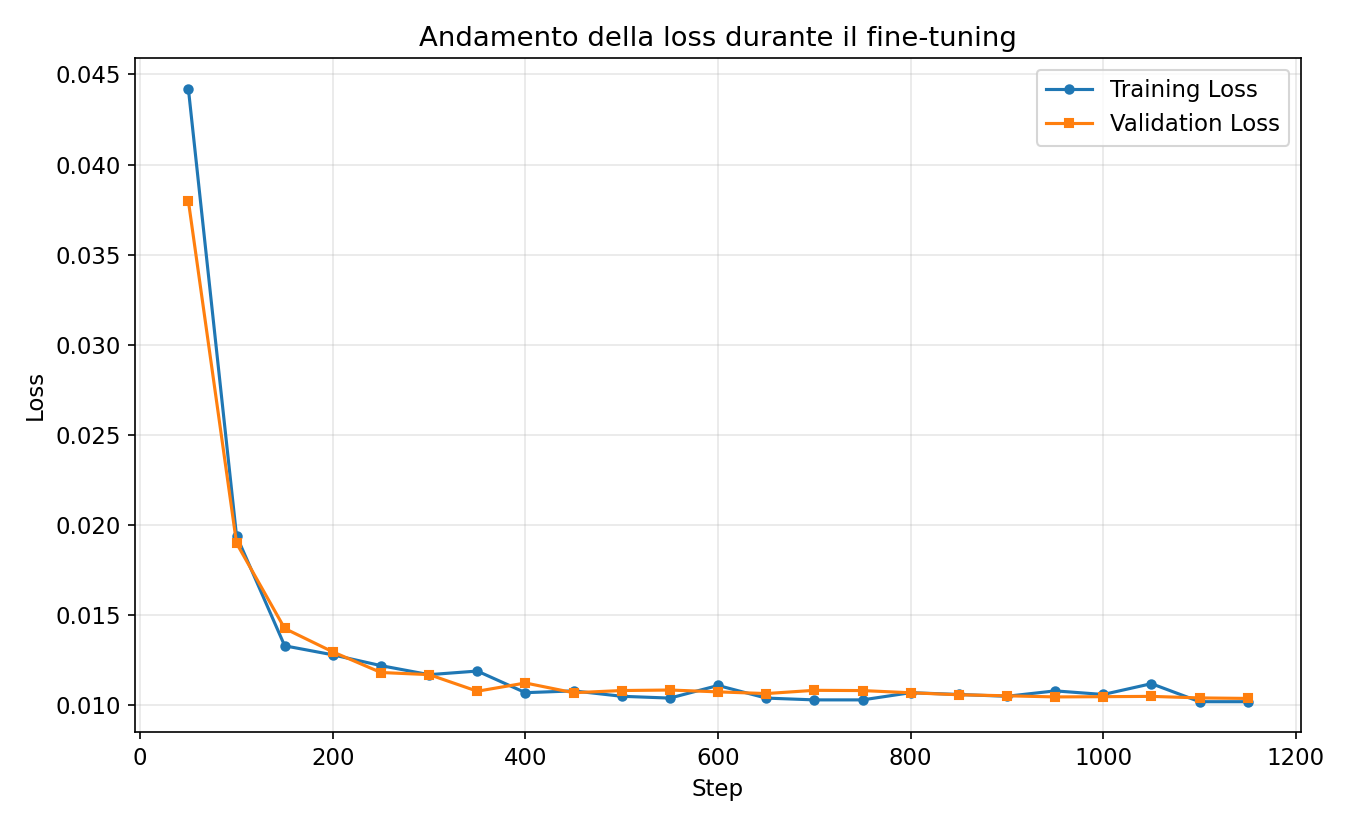
\includegraphics[width=0.85\textwidth]{../img/loss_curve.png}
\caption{Andamento della training loss e della validation loss durante il fine-tuning}\label{fig:loss_curve}
\end{figure}

La curva di \textit{validation loss} segue da vicino quella di training, senza divergenze significative: segno di assenza di overfitting. Entrambe le curve si stabilizzano già intorno allo step 400 su un totale di 1188, il che suggerisce che il modello avrebbe potuto convergere anche con meno step.

\newpage
\section{Efficacia: valutazione qualitativa}\label{sec:efficacia}


\subsection{Metriche di retrieval per categoria}\label{subsec:metriche_categoria}

Applicando la metodologia descritta in \cref{subsec:nota_metodologica}, ovvero il confronto sull'insieme completo dei risultati, al netto di \code{ORDER BY}/\code{LIMIT}, le metriche di precision, recall e F1 per categoria sono le seguenti:

\begin{table}[ht]
\centering
\begin{tabular}{lrrrr}
\toprule
Categoria & N & Precision & Recall & F1 \\
\midrule
data\_esatta        & 233 & 1.000 & 1.000 & 1.000 \\
formato\_file       & 66  & 1.000 & 1.000 & 1.000 \\
dispositivo         & 40  & 1.000 & 1.000 & 1.000 \\
container\_cartella & 30  & 1.000 & 1.000 & 1.000 \\
ricerca\_testuale   & 28  & 1.000 & 1.000 & 1.000 \\
autore              & 26  & 1.000 & 1.000 & 1.000 \\
data\_intervallo    & 20  & 1.000 & 1.000 & 1.000 \\
\midrule
\textbf{Media complessiva} & \textbf{443} & \textbf{1.000} & \textbf{1.000} & \textbf{1.000} \\
\bottomrule
\end{tabular}
\caption{Precision, recall e F1 medi per categoria, calcolati sull'insieme completo dei risultati (al netto di \code{ORDER BY}/\code{LIMIT})}\label{tab:metriche_categoria}
\end{table}

Anche il riconoscimento delle richieste Out-of-Domain (\cref{subsec:errori}) raggiunge il 100\% di accuratezza: tutti i 57 esempi fuori dominio nel test set sono stati correttamente classificati come tali dal modello. Allo stesso modo, il \code{limit\_match} (corrispondenza esatta del valore richiesto nella clausola \code{LIMIT}) è verificato nel 100\% dei 443 casi non Out-of-Domain in cui almeno una delle due query include un \code{LIMIT}.

\subsection{Nota critica: interpretazione dei risultati perfetti}\label{subsec:nota_critica}

I risultati riportati in \cref{tab:metriche_categoria} meritano una discussione esplicita, poiché un punteggio di 1.000 uniforme su ogni metrica e ogni categoria è un esito che richiede cautela interpretativa più che entusiasmo acritico.

Un'ispezione diretta delle 500 coppie (query generata, query di riferimento) in \code{predictions.json} rivela che \textbf{tutte le 500 query generate dal modello sono identiche, carattere per carattere, alla rispettiva query di riferimento}. Questo è un dato di fatto distinto, e più forte, della semplice equivalenza semantica dei risultati: non si tratta di formulazioni sintatticamente diverse che producono lo stesso insieme di risultati, ma di una riproduzione esatta della stringa SPARQL attesa.

Questo fenomeno è spiegabile alla luce di come il test set è stato costruito: le domande e le query di riferimento sono generate dallo stesso sistema di template parametrici (\cref{subsec:dataset_gen}) usato per produrre il dataset di training. Le 8 regole assolute del system prompt (\cref{subsec:regole}) vincolano fortemente la forma sintattica della query attesa: un'unica struttura \code{SELECT DISTINCT ?image WHERE \{\ldots\}}, predicati fissi per ciascun intento, che riduce lo spazio delle risposte plausibili a un insieme ristretto e, per costruzione, deterministico dato l'intento e i parametri della domanda.

In altre parole, una corrispondenza esatta al 100\% è coerente con due ipotesi non mutuamente esclusive:

\begin{enumerate}
    \item Il modello ha effettivamente appreso con grande efficacia la mappatura tra intenti linguistici e struttura SPARQL imposta dalle regole, generalizzando correttamente su parametri (anni, dispositivi, nomi di file) anche se non identici a quelli visti in training;
    \item Il test set, essendo generato dallo stesso processo del training set, condivide con esso una distribuzione di superficie sufficientemente vincolata (per via delle 8 regole assolute) da rendere il compito di generazione quasi deterministico, riducendo il valore di questa valutazione come misura di \emph{generalizzazione} a domande realmente nuove e formulate liberamente da un utente umano.
\end{enumerate}

Il codice di inferenza (\code{generate\_predictions.ipynb}) conferma che il test set costituisce una reale partizione \textit{held-out}: l'estrazione è avvenuta in modo deterministico con un rapporto 95\%/5\% e lo stesso seed (\code{3407}) usato per la configurazione del training. Questo esclude \textit{data leakage} o sovrapposizioni (il modello ha elaborato istanze mai viste in fase di addestramento) e avvalora l'ipotesi della generalizzazione strutturale (punto 1), pur confermando che tale generalizzazione avviene strettamente \textit{in-distribution} rispetto ai template.

Questa osservazione non invalida il risultato: un'accuratezza sintattica ed esecutiva del 100\% sui formati di query coperti dal generatore resta un traguardo solido e utile per l'applicativo. Ne delimita però la portata: la valutazione quantitativa qui presentata misura principalmente la capacità del modello di rispettare in modo affidabile e ripetibile la grammatica e le regole imposte dal system prompt, più che la sua capacità di decodificare formulazioni libere e impreviste di un ricercatore umano. Manca ancora una prova con domande poste in modo spontaneo da utenti reali, non vincolate dai template del generatore (\cref{chap:conclusioni}).

\subsection{Miglioramento rispetto alle soluzioni precedenti}\label{subsec:miglioramento}

Al di là delle metriche quantitative, l'efficacia del sistema si misura anche rispetto al miglioramento qualitativo delle funzionalità disponibili per il ricercatore umanista, in continuità con la discussione del \cref{chap:contesto} (architettura dell'informazione, berrypicking, carico cognitivo):

\begin{sloppypar}
\begin{itemize}
    \item \textbf{Funzionalità}: prima dell'introduzione del sistema, non esisteva alcun meccanismo di ricerca per contenuto o concetto sul Datavault; l'unica modalità di accesso era la navigazione diretta della struttura a container (\cref{subsec:dharc}). Il sistema introduce ex novo questa funzionalità.
    \item \textbf{Usabilità}: l'interazione è ridotta a un singolo campo di testo in linguaggio naturale, eliminando la necessità di conoscere prefissi RDF, sintassi SPARQL o la struttura interna dello schema (\cref{subsec:tre_barriere}).
    \item \textbf{Integrazione}: il sistema si integra nell'infrastruttura esistente (Fedora/Blazegraph) senza richiedere modifiche allo schema dati o migrazioni, operando come layer applicativo aggiuntivo.
    \item \textbf{Manutenzione}: la separazione netta tra dataset di training, system prompt e backend di inferenza (\cref{chap:implementazione}) consente di aggiornare il comportamento del sistema (ad esempio aggiungendo nuove categorie di query) senza dover intervenire sull'infrastruttura dati sottostante.
\end{itemize}
\end{sloppypar}

\subsubsection{Limite: nessun confronto diretto con l'alternativa manuale}

I quattro punti sopra restano un confronto qualitativo basato sull'analisi architetturale del sistema, non su una misura empirica diretta. Non è stato condotto né un cronometraggio del tempo necessario a un utente per scrivere manualmente le query SPARQL dei tre casi d'uso del \cref{chap:prototipo}, né un test di usabilità con ricercatori reali del dominio DH.ARC.\@

Un'indicazione indiretta della differenza attesa viene dalla complessità sintattica stessa dei casi d'uso discussi nel \cref{chap:prototipo}: query come quella del caso d'uso 3 (filtro multi-criterio su dispositivo, intervallo di date e formato) richiedono la conoscenza di almeno tre predicati RDF diversi (\code{exif:make}, \code{exif:dateTime}, \code{ebucore:hasMimeType}) e la sintassi corretta per combinarli in un unico \code{WHERE}, competenze che il profilo utente descritto nel \cref{subsec:utenti} tipicamente non possiede. Questo suggerisce che il vantaggio in termini di tempo e di soglia d'accesso sia sostanziale, ma resta appunto un'aspettativa qualitativa e non un dato misurato.

Colmare questa lacuna con un vero studio comparativo (a tempo, o con un gruppo di utenti reali) è indicato come sviluppo futuro nel \cref{chap:conclusioni}.

\section{Discussione dei risultati e limiti della valutazione}\label{sec:discussione}


I risultati di questo capitolo si riassumono in tre punti:

\begin{enumerate}
    \item Il sistema è \textbf{sintatticamente affidabile}: il 100\% delle query generate nel test set è eseguibile senza errori contro Blazegraph, grazie al vincolo imposto dalle 8 regole del system prompt.
    \item Il sistema è \textbf{efficiente nei tempi di risposta}: una media di 7.45 secondi per query su GPU T4 è compatibile con un'interazione conversazionale, sebbene il confronto con un'esecuzione su CPU richieda ulteriore verifica empirica (\cref{subsec:tempo_generazione}).
    \item I punteggi di precision/recall/F1 pari a 1.000 vanno interpretati con cautela metodologica (\cref{subsec:nota_critica}): riflettono primariamente la capacità del modello di rispettare un formato di query fortemente vincolato e generato dalla stessa famiglia di template del training set, più che una misura di generalizzazione su domande realmente libere.
\end{enumerate}

Il limite principale di questa valutazione è dunque la natura \textbf{sintetica e in-dominio} del test set utilizzato. Una valutazione più conclusiva richiederebbe un confronto con domande poste da utenti reali del dominio DH.ARC, non vincolate dalla struttura dei template di generazione: un'estensione discussa come sviluppo futuro nel \cref{chap:conclusioni}.

\section{Conclusioni del capitolo}\label{sec:conclusioni_cap5}


In questo capitolo abbiamo valutato il sistema lungo due assi complementari. Sul piano dell'\textbf{efficienza}, il sistema mostra tempi di generazione contenuti (media 7.45s su GPU), un tasso di esecuzione corretta del 100\% e una rapida convergenza in fase di training (loss stabilizzata già a circa un terzo del training totale). Sul piano dell'\textbf{efficacia}, le metriche di retrieval (precision, recall, F1) raggiungono il valore massimo su tutte le categorie testate: un risultato che, come discusso in \cref{subsec:nota_critica}, va attribuito principalmente all'efficacia delle regole di vincolo sintattico imposte dal system prompt e alla natura in-distribuzione del test set, più che a una dimostrata capacità di generalizzazione su input completamente liberi.

Il \cref{chap:conclusioni} riprende questi risultati per bilanciare i punti di forza del sistema con i suoi limiti noti, e per delineare gli sviluppi futuri necessari a una valutazione più rigorosa e a un utilizzo in produzione del sistema. 
\chapter{Conclusioni e sviluppi futuri}\label{chap:conclusioni}

\section{Introduzione al capitolo}\label{sec:intro_cap6}


I capitoli precedenti hanno definito il problema (\cref{chap:contesto}), presentato la soluzione (\cref{chap:prototipo}), descritto la sua realizzazione tecnica (\cref{chap:implementazione}) e misurato il suo comportamento (\cref{chap:valutazione}). Questo capitolo chiude il lavoro con un bilancio onesto: cosa il sistema realizza bene, dove restano margini di miglioramento, e perché rappresenti comunque un passo avanti rispetto alla situazione di partenza descritta nel \cref{chap:contesto}, ovvero l'sassenza totale di ricerca per contenuto o concetto sul Datavault.
Chiudiamo delineando gli sviluppi futuri, ordinati per priorità: dai bug fix più urgenti fino alle estensioni più ambiziose.

\section{Analisi critica del sistema}\label{sec:orgoglio_modestia}


\subsection{Risultati ottenuti e punti di forza}\label{subsec:punti_forza}

\subsubsection{Affidabilità sintattica}

Il risultato più solido del sistema è il tasso di esecuzione corretta del 100\% osservato sul test set held-out (\cref{subsec:tasso_esecuzione}): ogni query generata nel campione di valutazione è risultata eseguibile senza errori contro Blazegraph. Questo non è un dato scontato per un sistema basato su generazione di linguaggio: dimostra che il vincolo imposto dalle 8 regole assolute del system prompt (\cref{subsec:regole}), combinato con il fine-tuning su un dataset coerente con quelle stesse regole, produce un comportamento affidabile e ripetibile.

\subsubsection{Uno split di valutazione genuinamente held-out}

A differenza di molte valutazioni superficiali di sistemi basati su LLM, in questo lavoro è stato verificato esplicitamente, risalendo al codice di generazione delle predizioni (\cref{subsec:nota_critica}), che il test set non si sovrappone al training set. I 500 esempi valutati non sono mai stati osservati dal modello durante l'addestramento. Questo rigore metodologico, per quanto abbia comunque richiesto una discussione critica sulla natura in-distribuzione del test (\cref{subsec:nota_critica}), è di per sé un punto di forza: molti sistemi analoghi non documentano affatto come è stato costruito il proprio set di valutazione.





\subsubsection{Economicità delle risorse impiegate}

L'intera pipeline di addestramento (generazione del dataset sintetico, fine-tuning con LoRA, valutazione) è stata condotta con risorse gratuite (GPU T4 di Kaggle) e un modello di dimensioni contenute (Phi-3-mini, 3.8 miliardi di parametri). Il fine-tuning ha richiesto meno di 1200 step per raggiungere una loss stabile (\cref{subsec:convergenza}). Questo dimostra che un problema di dominio specifico e ben delimitato, come la traduzione da linguaggio naturale a una sintassi SPARQL vincolata, non richiede necessariamente modelli di grandi dimensioni o infrastrutture costose per essere affrontato efficacemente.

\subsubsection{Coerenza architetturale tra training e inferenza}

Il system prompt è identico, byte per byte, sia nel generatore del dataset sia nel backend di inferenza (\cref{subsec:regole}). Questa scelta, apparentemente minore, elimina una classe di errori comune nei sistemi basati su fine-tuning: il disallineamento tra le condizioni di addestramento e quelle di utilizzo reale (\textit{train-serve skew}).

\subsection{Limiti del sistema e criticità}\label{subsec:punti_modestia}

\subsubsection{Limiti della valutazione rispetto agli scenari d'uso reale}

Il limite più rilevante, discusso ampiamente nel \cref{subsec:nota_critica}, è che la valutazione quantitativa misura la capacità del modello di rispettare un formato di query generato dagli stessi template usati in training, non la sua capacità di gestire domande realmente libere, poste da un umanista che non conosce né le regole del sistema né le 13 categorie di query supportate (\cref{subsec:dataset_gen}). Nessun utente reale del dominio DH.ARC ha ancora interagito con il sistema in condizioni non controllate.

\subsubsection{Copertura parziale delle categorie nel test set}

Il generatore produce 13 categorie di query più la gestione Out-of-Domain, ma il test set effettivamente valutato ne copre solo 7 (\cref{subsec:distribuzione_test}). Categorie come la negazione (\code{query\_not\_anno}) o l'OR logico tra formati (\code{query\_or\_formati}) non sono rappresentate nel campione analizzato: non sappiamo con la stessa sicurezza se il sistema le gestisca altrettanto bene.

\subsubsection{Fragilità del sistema rispetto al bug del namespace EXIF}

La soluzione descritta in \cref{subsec:bug_exif_namespace} funziona, ma accoppia il sistema a un errore presente nei dati di produzione. Se il Datavault venisse in futuro corretto o migrato, sia il dataset di training sia il backend richiederebbero un aggiornamento sincronizzato: una dipendenza fragile che un sistema più maturo dovrebbe gestire in modo più robusto, ad esempio con un meccanismo di rilevamento automatico del namespace realmente in uso.

\subsubsection{Inferenza su CPU in produzione}

Il backend di produzione esegue l'inferenza su CPU (\cref{subsec:fastapi}), mentre i tempi di generazione misurati (\cref{subsec:tempo_generazione}) si riferiscono all'esecuzione su GPU T4. Non è stato misurato il tempo di risposta reale che un utente sperimenterebbe nell'uso quotidiano del sistema in produzione, un dato che sarebbe stato preferibile avere.

\subsubsection{Vincolo di lunghezza della sequenza}

Il limite di 1024 token in \code{max\_seq\_length} (\cref{subsec:hyperparams}), scelto per contenere l'uso di memoria durante il training, potrebbe risultare insufficiente per domande particolarmente articolate o per un futuro ampliamento del system prompt (ad esempio se si aggiungessero più predicati o esempi few-shot nel prompt stesso).

\subsection{Impatto e prospettive nel dominio umanistico}\label{subsec:giustificazione}

Rispetto alla situazione precedente, ovvero l'assenza di un meccanismo di ricerca per contenuto sul Datavault, con l'unica alternativa realistica rappresentata dalla scrittura manuale di SPARQL da parte di utenti privi delle competenze necessarie (\cref{subsec:tre_barriere}), il sistema sposta il problema da ``impossibile per l'utente target'' a ``possibile, con margini di miglioramento noti e documentati''. Non è una soluzione perfetta, ma è una soluzione \emph{funzionante} su un problema che, prima di questo lavoro, non aveva alcuna soluzione praticabile per un ricercatore umanista senza competenze SPARQL.\@



\section{Sviluppi futuri}\label{sec:sviluppi_futuri}


Gli sviluppi futuri sono organizzati in ordine di priorità decrescente: dai bug fix più urgenti alle estensioni più ambiziose.

\subsection{Bug fix}\label{subsec:bugfix}

\begin{enumerate}
    \item \textbf{Estendere la valutazione alle categorie mancanti}: eseguire la Fase 1/Fase 2 della pipeline di valutazione (\cref{subsec:metodologia}) su un campione che includa esplicitamente le categorie non rappresentate nel test set attuale (negazione, OR tra formati, paginazione custom, ricerca per uploader), per verificare se il tasso di esecuzione corretta del 100\% si mantiene anche lì.
    \item \textbf{Rendere il namespace EXIF configurabile}: estrarre il namespace hardcoded (\cref{subsec:bug_exif_namespace}) in un parametro di configurazione centralizzato, così che un'eventuale correzione futura del Datavault richieda una modifica in un solo punto anziché in due file separati.
    \item \textbf{Misurare i tempi di inferenza reali su CPU}: eseguire un benchmark diretto sul backend di produzione, sostituendo la stima qualitativa attuale (\cref{subsec:tempo_generazione}) con un dato misurato.
\end{enumerate}

\subsection{Feature mancanti}\label{subsec:feature_mancanti}

\begin{enumerate}
    \item \textbf{Un vero test di usabilità con utenti reali}: come discusso in \cref{subsec:miglioramento}, manca ancora una misura empirica del vantaggio percepito da un ricercatore umanista reale, sia in termini di tempo risparmiato sia di soddisfazione d'uso rispetto all'assenza di alternative.
    \item \textbf{Supporto multilingue}: il sistema opera attualmente solo in italiano. Un'estensione naturale, vista la composizione internazionale della comunità di ricerca in Digital Humanities, è l'aggiunta di supporto per l'inglese e altre lingue.
    \item \textbf{Un'interfaccia di correzione della query generata}: per gli utenti più esperti, permettere una modifica diretta della query SPARQL proposta dal sistema (già visualizzabile, si veda \cref{subsec:tre_layer}) prima dell'esecuzione, chiudendo il cerchio tra automazione e controllo manuale.
\end{enumerate}

\subsection{Estensioni fondamentali}\label{subsec:estensioni_fondamentali}

\begin{enumerate}
    \item \textbf{Ampliare la copertura semantica dello schema}: le 13 categorie attuali (\cref{subsec:dataset_gen}) coprono i pattern di ricerca più comuni rispetto all'attuale popolazione del Datavault, ma lo schema RDF contiene predicati non ancora sfruttati (ad esempio quelli PREMIS relativi alla dimensione dei file, o le relazioni RDFS di sottoclasse osservate nello schema). Un'estensione del dataset generativo potrebbe abilitare interrogazioni oggi non supportate.
    \item \textbf{Passare da un prompt statico a un vero meccanismo RAG dinamico}: il sistema attuale inietta lo schema RDF nel system prompt in forma fissa (\cref{subsec:regole}). Un'evoluzione naturale, discussa a livello teorico nel \cref{sec:rag}, è recuperare dinamicamente solo i frammenti di schema rilevanti per ciascuna domanda, permettendo al sistema di scalare a schemi più ampi o mutevoli senza dover ri-addestrare il modello a ogni modifica dell'ontologia.
    \item \textbf{Inferenza su GPU in produzione}: sostituire l'attuale deployment su CPU (\cref{subsec:fastapi}) con un'infrastruttura GPU dedicata, per ridurre i tempi di risposta percepiti dall'utente finale a un livello compatibile con un'interazione conversazionale fluida.
\end{enumerate}

\subsection{Possibili sviluppi futuri}\label{subsec:sviluppi_futuri}

\begin{enumerate}
    \item \textbf{Ricerca per contenuto visivo, non solo per metadati}: l'intero sistema attuale opera sui metadati EXIF, Dublin Core ed EBUCore associati alle immagini, non sul loro contenuto visivo. Un'estensione di grande ambizione sarebbe l'integrazione di modelli di visione (ad esempio embedding CLIP-like) che permettano domande come ``mostrami le immagini che raffigurano una miniatura con un drago'', andando oltre la ricerca per attributi tecnici o descrittivi verso una vera ricerca per concetto visivo, in piena coerenza con la visione di ``findability'' discussa nel \cref{chap:contesto}.
    \item \textbf{Un sistema federato su più Knowledge Graph}: estendere l'approccio oltre il singolo Datavault di DH.ARC, verso un'interrogazione federata di più triplestore appartenenti a istituzioni diverse del patrimonio culturale, con il sistema in grado di determinare autonomamente quali fonti interrogare per una data domanda.
    \item \textbf{Apprendimento continuo dal feedback degli utenti}: un meccanismo di active learning che raccolga le correzioni manuali degli utenti esperti (si veda il punto sull'interfaccia di correzione, \cref{subsec:feature_mancanti}) per arricchire iterativamente il dataset di training e migliorare il modello nel tempo, senza richiedere una nuova generazione sintetica da zero.
\end{enumerate}

\section{Conclusioni finali}\label{sec:conclusioni_finali}


Questo lavoro nasce da un'osservazione semplice: il Datavault di DH.ARC contiene milioni di triple RDF, ma nessun modo agile per ricercatori umanisti di interrogarle se non conoscendo SPARQL.\@ Abbiamo affrontato questo problema costruendo un LLM Query Builder che traduce domande in linguaggio naturale italiano in query SPARQL valide, attraverso il fine-tuning di un modello di dimensioni contenute su un dataset sintetico costruito appositamente per il dominio.

I risultati raccolti nel \cref{chap:valutazione} mostrano un sistema sintatticamente affidabile, efficiente nei tempi di generazione e coerente nella sua architettura tra fase di training e fase di inferenza. Allo stesso tempo, la discussione onesta dei suoi limiti (una valutazione ancora in-distribuzione, l'assenza di un test con utenti reali, la fragilità nota rispetto ai dati di produzione) delimita la portata di quanto qui dimostrato, senza sminuire il fatto che Datavault dispone di un meccanismo di ricerca per contenuto praticabile da chi non conosce SPARQL.\@

Gli sviluppi futuri delineati in questo capitolo, dalla verifica delle categorie non ancora testate fino alla visione più ambiziosa di una ricerca per contenuto visivo, tracciano un percorso che potrebbe portare ad un significativo miglioramento in termini di efficacia e usabilità del sistema. 










\renewcommand{\bibsection}{}
\chapter*{Riferimenti bibliografici}
\addcontentsline{toc}{chapter}{Riferimenti bibliografici}
\nocite{*}   \bibliography{../refs}
\newpage




\newpage~\newpage
\chapter*{Ringraziamenti}
Grazie a tutt*.

\end{document}
